\documentclass[a4paper,12pt,times,numbered,print,index,spanish]{Classes/PhDThesisPSnPDF}
%~ Aca agrego ,chapter o ,abstract para solo imprimir el abstract o algun capitulo en particular

%~ \usepackage[spanish]{babel}
\usepackage[utf8]{inputenc}



% Preamble: Contains packages and user-defined commands and settings
%~ Este es importante, lo dejo como está
% ******************************************************************************
% ****************************** Custom Margin *********************************

% Add `custommargin' in the document class options to use this section
% Set {innerside margin / outerside margin / topmargin / bottom margin}  and
% other page dimensions
\ifsetCustomMargin
  \RequirePackage[left=37mm,right=30mm,top=35mm,bottom=30mm]{geometry}
  \setFancyHdr % To apply fancy header after geometry package is loaded
\fi

% *****************************************************************************
% ******************* Fonts (like different typewriter fonts etc.)*************

% Add `customfont' in the document class option to use this section

\ifsetCustomFont
  % Set your custom font here and use `customfont' in options. Leave empty to
  % load computer modern font (default LaTeX font).
  \RequirePackage{helvet}
\fi

% *****************************************************************************
% **************************** Custom Packages ********************************

% ************************* Algorithms and Pseudocode **************************

%\usepackage{algpseudocode}


% ********************Captions and Hyperreferencing / URL **********************

% Captions: This makes captions of figures use a boldfaced small font.
%\RequirePackage[small,bf]{caption}

\RequirePackage[labelsep=space,tableposition=top]{caption}
\renewcommand{\figurename}{Fig.} %to support older versions of captions.sty


% *************************** Graphics and figures *****************************

%\usepackage{rotating}
%\usepackage{wrapfig}

% Uncomment the following two lines to force Latex to place the figure.
% Use [H] when including graphics. Note 'H' instead of 'h'
%\usepackage{float}
%\restylefloat{figure}

% Subcaption package is also available in the sty folder you can use that by
% uncommenting the following line
% This is for people stuck with older versions of texlive
%\usepackage{sty/caption/subcaption}
\usepackage{subcaption}

% ********************************** Tables ************************************
\usepackage{booktabs} % For professional looking tables
\usepackage{multirow}

%\usepackage{multicol}
%\usepackage{longtable}
%\usepackage{tabularx}


% ***************************** Math and SI Units ******************************

\usepackage{amsfonts}
\usepackage{amsmath}
\usepackage{amssymb}
\usepackage{siunitx} % use this package module for SI units


% ******************************* Line Spacing *********************************

% Choose linespacing as appropriate. Default is one-half line spacing as per the
% University guidelines

% \doublespacing
% \onehalfspacing
% \singlespacing


% ************************ Formatting / Footnote *******************************

% Don't break enumeration (etc.) across pages in an ugly manner (default 10000)
%\clubpenalty=500
%\widowpenalty=500

%\usepackage[perpage]{footmisc} %Range of footnote options


% *****************************************************************************
% *************************** Bibliography  and References ********************

%\usepackage{cleveref} %Referencing without need to explicitly state fig /table

% Add `custombib' in the document class option to use this section
\ifuseCustomBib
   \RequirePackage[square, sort, numbers, authoryear]{natbib} % CustomBib

% If you would like to use biblatex for your reference management, as opposed to the default `natbibpackage` pass the option `custombib` in the document class. Comment out the previous line to make sure you don't load the natbib package. Uncomment the following lines and specify the location of references.bib file

%\RequirePackage[backend=biber, style=numeric-comp, citestyle=numeric, sorting=nty, natbib=true]{biblatex}
%\bibliography{References/references} %Location of references.bib only for biblatex

\fi

% changes the default name `Bibliography` -> `References'
\renewcommand{\bibname}{References}


% *****************************************************************************
% *************** Changing the Visual Style of Chapter Headings ***************
% This section on visual style is from https://github.com/cambridge/thesis

% Uncomment the section below. Requires titlesec package.

%\RequirePackage{titlesec}
%\newcommand{\PreContentTitleFormat}{\titleformat{\chapter}[display]{\scshape\Large}
%{\Large\filleft{\chaptertitlename} \Huge\thechapter}
%{1ex}{}
%[\vspace{1ex}\titlerule]}
%\newcommand{\ContentTitleFormat}{\titleformat{\chapter}[display]{\scshape\huge}
%{\Large\filleft{\chaptertitlename} \Huge\thechapter}{1ex}
%{\titlerule\vspace{1ex}\filright}
%[\vspace{1ex}\titlerule]}
%\newcommand{\PostContentTitleFormat}{\PreContentTitleFormat}
%\PreContentTitleFormat


% ******************************************************************************
% ************************* User Defined Commands ******************************
% ******************************************************************************

% *********** To change the name of Table of Contents / LOF and LOT ************

%\renewcommand{\contentsname}{My Table of Contents}
%\renewcommand{\listfigurename}{My List of Figures}
%\renewcommand{\listtablename}{My List of Tables}


% ********************** TOC depth and numbering depth *************************

\setcounter{secnumdepth}{2}
\setcounter{tocdepth}{2}


% ******************************* Nomenclature *********************************

% To change the name of the Nomenclature section, uncomment the following line

%\renewcommand{\nomname}{Symbols}


% ********************************* Appendix ***********************************

% The default value of both \appendixtocname and \appendixpagename is `Appendices'. These names can all be changed via:

%\renewcommand{\appendixtocname}{List of appendices}
%\renewcommand{\appendixname}{Appndx}

% ******************************** Draft Mode **********************************

% Uncomment to disable figures in `draftmode'
%\setkeys{Gin}{draft=true}  % set draft to false to enable figures in `draft'

% These options are active only during the draft mode
% Default text is "Draft"
%\SetDraftText{DRAFT}

% Default Watermark location is top. Location (top/bottom)
%\SetDraftWMPosition{bottom}

% Draft Version - default is v1.0
%\SetDraftVersion{v1.1}

% Draft Text grayscale value (should be between 0-black and 1-white)
% Default value is 0.75
%\SetDraftGrayScale{0.8}


%% Todo notes functionality
%% Uncomment the following lines to have todonotes.

%\ifsetDraft
%	\usepackage[colorinlistoftodos]{todonotes}
%	\newcommand{\mynote}[1]{\todo[author=kks32,size=\small,inline,color=green!40]{#1}}
%\else
%	\newcommand{\mynote}[1]{}
%	\newcommand{\listoftodos}{}
%\fi

% Example todo: \mynote{Hey! I have a note}


% ************************ Thesis Information & Meta-data **********************
% Thesis title and author information, refernce file for biblatex
% ************************ Thesis Information & Meta-data **********************
\title{Estudios sobre la regulación de la expresión génica por microARNs en plantas mediante estrategias bioinformáticas}
%~ \subtitle{Using the CUED template}

%% The full name of the author
\author{Presentada por: Uciel Pablo Chorostecki}

\lugar{Rosario, Argentina}

%% Department (eg. Department of Engineering, Maths, Physics)
%~ \dept{Department of Engineering}

%% University and Crest
\university{Facultad de Ciencias Bioquímicas y Farmacéuticas - Universidad Nacional de Rosario}
\crest{
\includegraphics[width=0.3\textwidth]{logo_unr}}

%% Full title of the Degree
\degreetitle{Tesis de Doctorado}


%% Submission date
% Default is set as {\monthname[\the\month]\space\the\year}
%\degreedate{September 2014} 

%% Meta information
\subject{LaTeX} \keywords{{Tesis} {Bioinformatica} {UNR} {microARNs}}



%~ Esto solo sirve por si quiero imprimir solo el abstract o algun capitulo

% ***************************** Abstract Separate ******************************
% To printout only the titlepage and the abstract with the PhD title and the
% author name for submission to the Student Registry, use the `abstract' option in
% the document class.

\ifdefineAbstract
 \pagestyle{empty}
 \includeonly{Declaration/declaration, Abstract/abstract}
\fi

% ***************************** Chapter Mode ***********************************
% The chapter mode allows user to only print particular chapters with references
% Title, Contents, Frontmatter are disabled by default
% Useful option to review a particular chapter or to send it to supervisior.
% To use choose `chapter' option in the document class

\ifdefineChapter
 \includeonly{Chapter3/chapter3}
\fi

%~ Esto solo sirve por si quiero imprimir solo el abstract o algun capitulo

% ******************************** Front Matter ********************************
\begin{document}

\frontmatter

\begin{titlepage}
  \maketitle
\end{titlepage}

% ******************************* Thesis Declaration ***************************

\begin{declaration}

\begin{center}

{\Large \bfseries{Estudios sobre la regulación de la expresión génica por microARNs en plantas mediante estrategias bioinformáticas} \par} 
\vspace*{3em}

{\Large Uciel Pablo Chorostecki \par} 
\vspace*{2em}
{\Large Licenciado en Ciencias de la Computación \par} 
\vspace*{.5em}
{\Large Universidad Nacional de Rosario\par} 
\vspace*{3em}

\end{center}


Esta Tesis es presentada como parte de los requisitos para optar al grado académico de Doctor en Ciencias Biológicas, 
 de la Universidad de Rosario y no ha sido presentada previamente para la obtención de otro título en esta u otra Universidad. 
 La misma contiene los resultados obtenidos en investigaciones llevadas a cabo en el Instituto de Biología Molecular y Celular de Rosario (IBR-CONICET),
 dependiente de la Facultad de Cs. Bioquímicas y Farmacéuticas, durante el período comprendido entre Abril de 2012 y Marzo de 2016, 
 bajo la dirección del Dr. Javier Palatnik.



\end{declaration}


% ******************************* Thesis Dedidcation ********************************

\begin{dedication} 

I would like to dedicate this thesis to my loving parents \dots

\end{dedication}


%~ % ************************** Thesis Acknowledgements **************************

\begin{acknowledgements}      


And I would like to acknowledge ...
%~ Director
%~ compañeros de grupo
%~ Familia
%~ Amigos
%~ Tutores
%~ Colaboradores
%~ Director en BCN
%~ Conicet agencia por el apoyo económico
%~ Embo, IUBMB por las becas otorgadas para mi perfeccionamiento y trabajo en Nápoles y Barcelona.
%~ Tato? libreciencia?

\end{acknowledgements}


% *********************** Adding TOC and List of Figures ***********************

\tableofcontents

\listoffigures

\listoftables

% \printnomencl[space] space can be set as 2em between symbol and description
%\printnomencl[3em]

% ************************** Thesis Abstract *****************************
% Use `abstract' as an option in the document class to print only the titlepage and the abstract.
\renewcommand{\chaptername}{Abstract}

\begin{abstract}
Los microARNs (o miARNs) son ARN no codificantes que regulan la expresión génica en animales y plantas, y están implicados en procesos biológicos muy variables, como el desarrollo, la diferenciación y el metabolismo.
Con un largo de aproximadamente 21 nucleótidos, los miARNs reconocen secuencias parcialmente complementarias en los ARNm blanco, provocando su corte o arresto de la traducción.
Los miARNs han saltado rápidamente a la primera plana del interés de la comunidad científica como un nuevo nivel en el control de la expresión génica en eucariotas.
Estudios recientes han puesto de manifiesto que los miARNs están implicados en distintas patologías de seres humanos.
Los cálculos actuales consideran que cerca del 40\% de los genes de humanos se encuentran regulados por miARNs. 

Está generalmente aceptado que los miARNs en plantas tienen una extensiva complementariedad con sus genes blanco y su predicción por lo general se basa en el uso de parámetros empíricos deducidos de interacciones conocidas y validadas experimentalmente.
En este trabajo, primero desarrollamos una estrategia para la identificación de genes blanco regulados por miARNs en plantas, basado en la conservación evolutiva del par miARN-gen blanco.
Además, pudimos encontrar genes blanco específicos de Solanaceae y demostrar que la estrategia se puede utilizar para la búsqueda de genes blanco pertenecientes a un grupo determinado de especies.
Esta estrategia fue usada para predecir nuevas interacciones no conocidas anteriormente en \textit{Arabidopsis thaliana}, que luego fueron validados experimentalmente.
Algunos de los nuevos genes identificados podrían participar de las mismas vías que genes blanco conocidos anteriormente, sugiriendo que algunos miARNs pueden controlar diferentes aspectos de un proceso biológico.

A partir de estos resultados, desarrollamos una herramienta bioinformática disponible en un servidor de acceso público para identificar genes blanco de miARNs basada principalmente en la conservación durante la evolución de la interacción del par miARN-gen blanco en distintas especies.
La herramienta también brinda una descripción de varios parámetros de las interacciones miARN-gen blanco en distintas especies, que puede ser útil para mejorar los sistemas de predicción y describir la co-evolucion de los miARNs y los genes blanco. 

La biogénesis de los miARNs es un proceso clave porque determina la secuencia exacta de nucleótidos del ARN pequeño funcional, que luego determina los genes a ser regulados. 
Los precursores de miARNs de plantas son muy variables en forma y tamaño en comparación con los precursores de miARNs de plantas.
Y por lo tanto, poco se sabía sobre el reconocimiento de los precursores por la maquinaria de procesamiento.
En la segunda parte de este trabajo presentamos una estrategia para estudiar la conservación de los precursores de miARNs de plantas en distintas especies identificando regiones y dominios presentes en distintas especies.
A partir de estos resultados, desarrollamos un herramienta de visualización para poder analizar fácilmente la conservación de la estructura primaria y secundaria de los precursores de miARNs.
El análisis las mismas reveló que existe una marcada correlación entre la conservación de los precursores y el mecanismo de procesamiento.
Los resultados muestran patrones de conservación en los dominios necesarios para el procesamiento, y permiten deducir un modelo general del reconocimiento del ARN durante la biogénesis de miARNs.

\end{abstract}


\printnomencl

% ******************************** Main Matter *********************************
\mainmatter

\renewcommand{\chaptername}{Capítulo}
%~ \renewcommand{\figurename}{Figura}


\graphicspath{{Chapter1/Figs/}}

\setcounter{chapter}{4}
\chapter*{Resultados y Discusión Capítulo 1} 
\addcontentsline{toc}{chapter}{Resultados y Discusión Capítulo 1}


{\LARGE Aplicaciones bioinformáticas para el estudio de interacciones miARN-gen blanco}

\section{Introducción}
%~ patmatch del TAIR es utilizado para...
Los miARNs son ARN pequeños de alrededor de 21 nucleótidos, son importantes reguladores de la expresión de genes en eucariotas y controlan procesos claves como el desarrollo y la respuesta a estrés.
Los miARNs es controlan la expresión génica ajustando los niveles finales de las proteínas o eliminando los transcriptos de ARN en la célula.
La identidad de los genes blancos está especificada por la molécula de miARN, la cual reconoce una secuencia por complementariedad de bases. 
En plantas, los miARNs tienen una buena complementariedad con sus blancos y en muchos casos regulan más de un gen de una misma familia \citep{Jones-Rhoades2006}.

Los miARNs conservados en plantas se encuentran generalmente como pequeñas familias de genes que codifican ARN pequeños de secuencias similares o idénticas (Figura \ref{fig:variabilidad_maduro}).
Una de las ventajas de tener familias génicas con múltiples miembros es que proporciona flexibilidad en la manera en la que cada uno de ellos es regulado \citep{pmid21466971, pmid19699140}.
Estas diferencias pueden ser por variaciones en elementos regulatorios en los promotores o en las estructuras de los precursores de miARNs que llevan a eficiencias de procesamiento diferenciales \citep{pmid19699140}.

Por otro lado, las diferencias en las secuencias de los miARNs maduros podrían causar que miARNs de una misma familia regulen diferentes conjuntos de genes.
Esto se ha demostrado previamente para los miARNs miR319 y miR159.
Estos dos miARNs son muy similares en secuencia, al punto que varios autores los consideran miembros de una misma familia \citep{Jones-Rhoades2006}.
Sin embargo ha sido demostrado que regulan genes diferentes \citep{Schwab2005517, pmid12931144,Palatnik2007}.
Así, mientras el miR319 puede reprimir la expresión de factores de transcripción de la familia TCP y MYB, diferencias de secuencia en 4 nucleótidos previenen la actividad del miR159 sobre los TCP \citep{Palatnik2007}.

La identificación de genes blanco regulados por miARNs en plantas es muy importante para poder conocer el rol de los miARNs.
En general está identificación de genes blanco, se obtiene de diferentes estrategias computacionales donde tienen en cuenta la complementariedad con sus mensajeros blanco.
Un de los mayores desafío ha sido poder encontrar la mayoría de los genes regulados por estos ARN pequeños con una baja frecuencia de predicciones falsas.

A partir de predicciones de genes blanco y luego validación experimental, se han determinado algunos parámetros empíricos para la identificación de genes blanco.
Por un lado, el hecho de que determinados genes con un número de "mismatches" fuesen blancos de regulación por miARNs mientras que otros con igual número no, sugería que debían existir otros factores que afectaran la interacción de los miARN con los ARNm blanco.
Es por esto que se han utilizado otros enfoques para abordar este problema, por ejemplo el requerimiento de que el sitio complementario al miARN en los ARNm estuviera conservados entre genes homólogos de Arabidopsis y arroz.

Más recientemente se desarrolló una tecnología, en este caso experimental, conocida como "degradoma", que permite obtener el perfil global de los productos de degradación de los ARN mensajeros \citep{German2008,pmid18472421}.
Este enfoque permitió detectar in vivo y a nivel genómico la actividad de los miARNs al identificarse los productos de corte de los ARNm mediado por estos ARNs pequeños.
Dicha información es muy útil para la identificación de nuevos posibles blancos.

En esta parte de la Tesis se profundizó esta cuestión y se desarrolló un método bioinformático para la predicción de genes regulados por miARNs conservados en plantas.


\begin{figure}[htbp!] 
    \centering    
    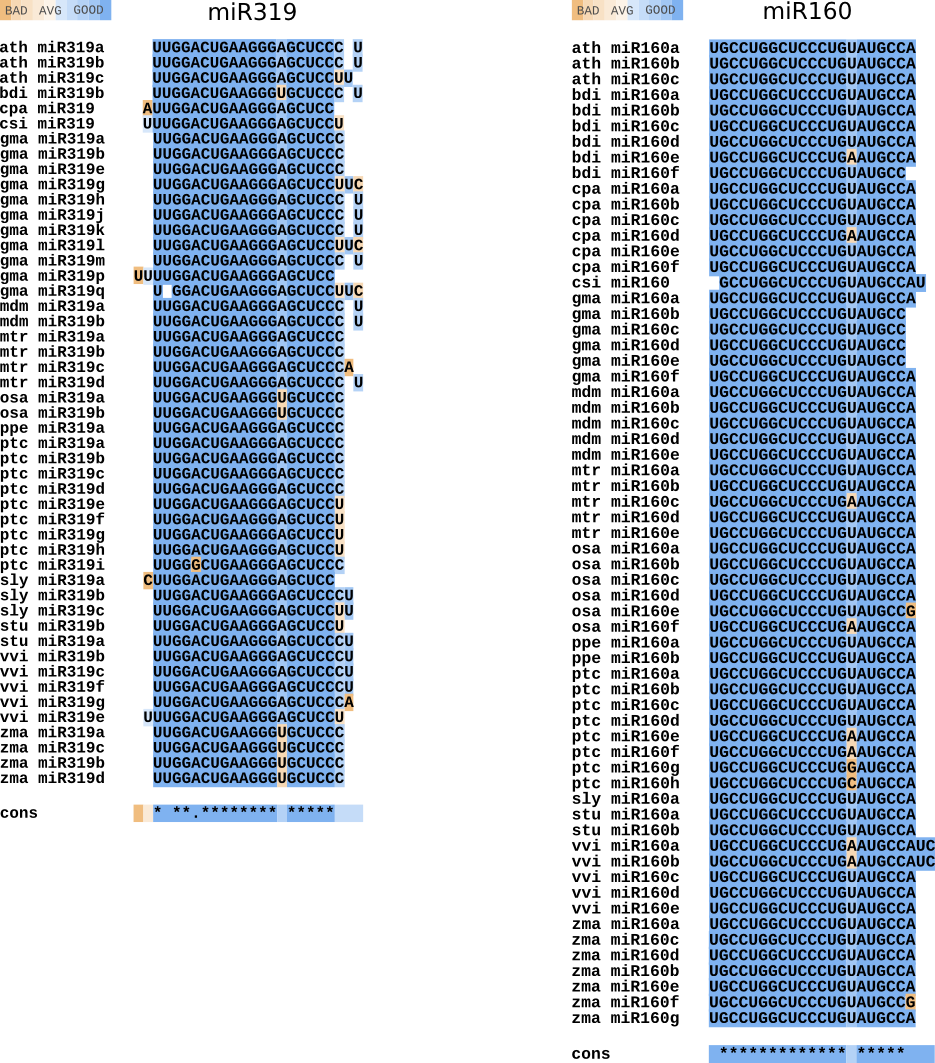
\includegraphics[width=0.7\textwidth]{variabilidad_maduro.png}
    \caption[Variabilidad de la secuencia del maduro]{
    Variabilidad de la secuencia del maduro.
		}
    \label{fig:variabilidad_maduro}
\end{figure}


\section{Resultados y Discusión}

\subsection{Predicción de genes regulados por miARNs.} %Section - 1.1 
\subsubsection{Diseño de una estrategia para la identificación de genes blanco regulados por miARNs basado en la conservación evolutiva del par miARN-gen blanco.}

Enfocamos nuestro análisis en 22 miARNs que están conservados en Angiospermas \citep{citeulike:8816489,10.1371/journal.pgen.1002419}.
En general estos miARNs están codificados por pequeñas familias hasta 32 miembros.
En los genomas completos de Arabidopsis, poplar y arroz es común encontrar variaciones en la secuencia de los miARNs pertenecientes a una misma familia, especialmente en el primer nucleótido y los nucleótidos 20 y 21 \citep{10.1371/journal.pgen.1002419}.

Sin embargo, observamos que la región entre la posición 2 y 19 está bastante conservada y pudimos encontrar una secuencia consenso presente en la mayoría de los miembros de cada familia de miARNs en esas tres especies (tabla \ref{table:table_consensus}).
Curiosamente, las bases variables fuera de esta región conservada son propensas a tener "mismatches" con genes blanco conocidos, lo que indica que podría existir una correlación entre la interacción miARN-gen blanco y la conservación de la secuencia del miARN.

Diseñamos una estrategia para identificar nuevos pares miARN-gen blanco principalmente basada en la conservación evolutiva de la secuencia del gen blanco (Figura \ref{fig:NAR_fig1}).
Las secuencias consenso de 18 nt de cada familia de miARN fueron usadas inicialmente para realizar la búsqueda de genes blanco en contigs de ESTs, de 41 especies de plantas, obtenidos de “Gene Index Project” un proyecto mantenido y administrado por la universidad de Harvard que contiene un catálogo completo de genes en una amplia gama de organismos incluyendo plantas.
Además se utilizaron ARNm completos para \textit{A. thaliana} y \textit{Oryza Sativa} para ver la lista completa de especies, ver tabla \ref{table:NAR_table_S2}).
Utilizando las secuencias consenso de 18nt y permitiendo 3 "mismatches", la búsqueda de genes blanco arrojó como resultado 38.597 genes distribuídos en las 43 especies (Figura \ref{fig:NAR_fig1}, bin 1).
Las interacciones G-U y los bulges fueron considerados como "mismatches" en esta primera búsqueda. Todos los genes blanco de  \textit{A. thaliana} conocidos hasta ese momento fueron identificados usando esta estrategia con la excepción de CSD2, un gen blanco del miR398 que contiene 4 mismatches ( tabla \ref{table:NAR_table_S2}).

Teniendo en cuenta que la mayoría de los genes blanco arrojados presentan una escasa descripción del tipo genómica funcional, realizamos un BLASTx  contra el proteoma de \textit{A. thaliana}.
El "locus ID" obtenido como "best hit" se utilizó como tag (etiqueta) para identificar al candidato en distintas especies (Figura \ref{fig:NAR_fig1}).
A pesar que esta estrategia no necesariamente identifica el gen ortólogo de Arabidopsis, sirve como propósito de clasificación de cada potencial gen blanco de miARN.
Aunque la mayoría de los potenciales genes blanco pudieron ser fácilmente asignados con una etiqueta, algunos pocos casos, que incluye a los genes que representan ARNs no codificantes fueron perdidos en este paso.

Este enfoque permite la selección de los mejores candidatos basándose en la presencia de los genes blanco en un número distinto de especies.
Utilizando 4 especies como el mínimo de especies requeridas (ya que tiene una buena especificidad), dio como resultado 3.781 genes que corresponden a 533 tags diferentes (Figura \ref{fig:NAR_fig1}, bin 2).

La búsqueda también se puede hacer en combinación con filtros empíricos de interacción par miARN-gen blanco que tienen en cuenta la energía de interacción y la posición de los "mismatches" (ver Materiales y métodos).
De los 38.597 candidatos iniciales, 9.375 pasan estos filtros (Figura \ref{fig:NAR_fig1}, bin 4).
Combinando filtros de energía y filtro de conservación evolutiva, la búsqueda arrojó como resultado 563 candidatos correspondientes a 146 tags (Figura \ref{fig:NAR_fig1}, bin 5).


\begin{figure}[htbp!] 
    \centering    
    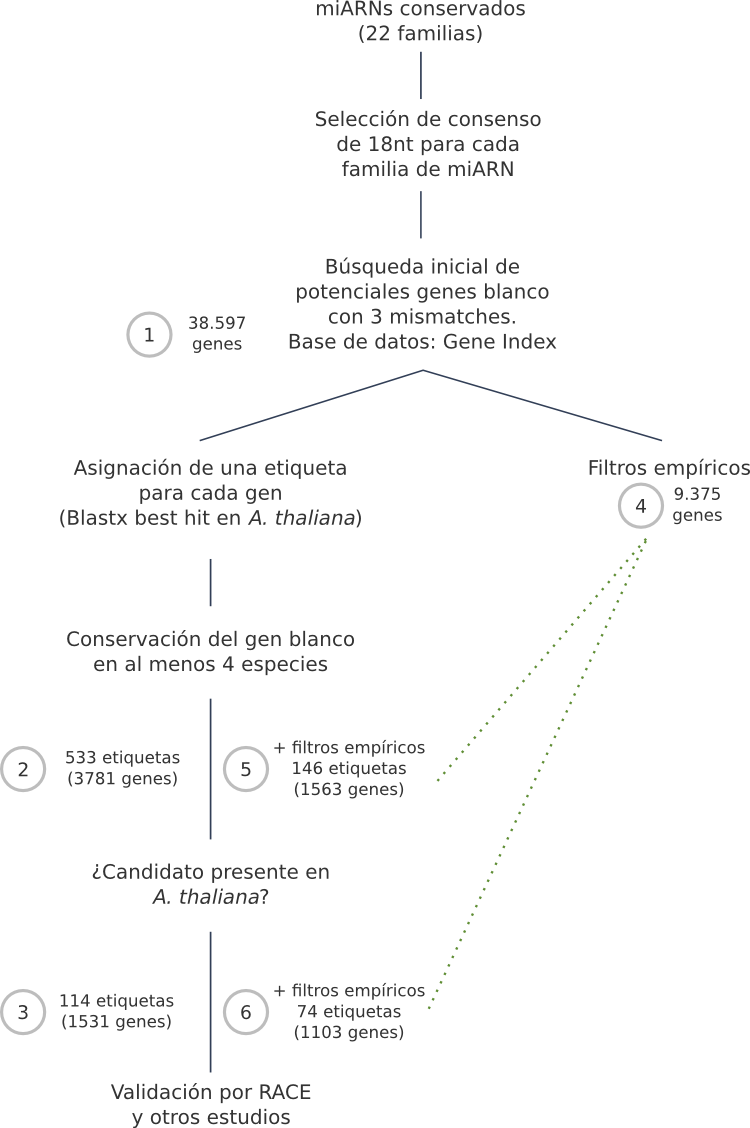
\includegraphics[width=0.7\textwidth]{NAR_fig1.png}
    \caption[Estrategia]{Esquema de la estrategia para la identificación de nuevos genes blanco.
    El número de genes blanco está identificado en cada paso. 
    Luego de aplicar el análisis de conservación, todos los genes que tienen el mismo hit en Arabidopsis, fueron considerados como un solo gen blanco. 
    El lado derecho muestra la búsqueda hecha con filtros empíricos: bin 5 y 6 incluyen genes blanco seleccionados con ambos filtros, empíricos y de conservación.
    Mientras que el bin 2 y 3 muestra los potenciales genes blanco seleccionados sólo con el filtro de conservación.}
    \label{fig:NAR_fig1}
\end{figure}



\begin{table}
\tiny
\centering
\caption{miARNs y sus genes blanco en plantas}
\label{table:table_consensus}
\begin{tabular}{lllll}
\hline
\textbf{miARN} & \textbf{Consenso (18 nt)} & \textbf{Targets conocidos$^{(a,b)}$} &  &  \\ \hline
miR156 & GACAGAAGAGAGTGAGCA & factores de transcripción SPL&  &  \\
miR159 & TTGGATTGAAGGGAGCTC & factores de transcripción MYB, \textbf{NOZZLE (NZL)}&  &  \\
miR160 & GCCTGGCTCCCTGTATGC & factores de transcripción ARF&  &  \\
miR162 & CGATAAACCTCTGCATCC & DCL1&  &  \\
miR164 & GGAGAAGCAGGGCACGTG & factores de transcripción NAC&  &  \\
miR166 & CGGACCAGGCTTCATTCC & factores de transcripción HDZip&  &  \\
miR167 & GAAGCTGCCAGCATGATC & factores de transcripción ARF, \textbf{IAA-ALANINE RESISTANT 3 (IAR3)}&  &  \\
miR168 & CGCTTGGTGCAGGTCGGG & AGO1&  &  \\
mir169 & AGCCAAGGATGACTTGCC & factores de transcripción CCAAT-HAP2&  &  \\
mir171 & TTGAGCCGTGCCAATATC & factores de transcripción GRAS&  &  \\
miR172 & GAATCTTGATGATGCTGC & factores de transcripción AP2&  &  \\
miR319 & TGGACTGAAGGGAGCTCC & factores de transcripción TCP&  &  \\
miR390 & AGCTCAGGAGGGATAGCG & TAS RNA&  &  \\
miR393 & CCAAAGGGATCGCATTGA & TIR1 proteins, F-BOX proteins&  &  \\
miR394 & TGGCATTCTGTCCACCTC & proteínas F-BOX &  &  \\
miR395 & TGAAGTGTTTGGGGGAAC & ATP-sulfurilasas, transportadores de sulfato&  &  \\
miR396 & TCCACAGCTTTCTTGAAC & factores de transcripción GRF, \textbf{MMG4.7, FLUORESCENT IN BLUE LIGHT (FLU)}&  &  \\
miR397 & CATTGAGTGCAGCGTTGA & Laccases&  &  \\
miR398 & GTGTTCTCAGGTCACCCC & Cu/Zn SODs, CytC oxidase protein subunit, Chaperona de cobre (CCS)&  &  \\
miR399 & GCCAAAGGAGATTTGCCC & Enzima E2 de conjugación de ubiquitina&  &  \\
miR408 & TGCACTGCCTCTTCCCTG & Blue copper proteins, Laccases, \textbf{P-TYPE ATPase (PAA2), PAC1 (Proteasome component)}&  &  \\
miR827 & TAGATGACCATCAGCAAA & SPX proteins&  &  \\ \hline
\multicolumn{3}{l}{a Los genes blanco fueron agrupados según sus funciones.}\\
\multicolumn{3}{l}{b Nuevos genes blanco validados experimentalmente en este estudio están indicados en negrita.}\\

\end{tabular}
\end{table}

\subsubsection{Parámetros empíricos y de conservación evolutiva pueden actuar de manera sinérgica para identificar genes blanco regulados por miARNs.}
Potenciales genes blanco de miARNs fueron clasificados de acuerdo al mínimo número de especie en donde fueron detectados (Figura 2A-E).
Como control para cada miARN generamos 10 secuencias “scramble” (al azar), dividiendo las secuencias originales de a di-nucleótidos y luego generando nuevas secuencias al azar conservando la composición de los di-nucleótidos.
Estas secuencias al azar fueron utilizadas para realizar búsqueda de genes blanco del mismo modo que lo hicimos para las secuencias originales.
La relación señal/ruido fue calculada como el cociente entre el número de genes blanco para los miARNs y el número promedio obtenido de las secuencias al azar.
El radio fue de 1,2 para todos los miARNs juntos sin requerir conservación y esa relación incrementa con el número de especie en donde los genes blanco fueron detectados (Figura \ref{fig:NAR_fig2} A, recuadro). 
Los datos para todos los miARNs y sus potenciales genes blanco conservados en al menos 4 especies están incluidos en la tabla \ref{table:NAR_table_2}.

Luego estudiamos la selección de candidatos teniendo en cuenta los filtros empíricos.
Para esto aplicamos una versión modificada de los filtros descritos anteriormente y requiriendo (i) una energía mínima de hibridación (MFE) de al menos 72\% del apareamiento perfecto de cada secuencia consenso y (ii)  que sólo un "mismatch" pudiera estar presente entre la posición 1 y la 11 de la secuencia consenso (2-12 del miARN).
De la búsqueda inicial 9.375 genes pasaron estos filtros conteniendo el 97\% de los genes validados anteriormente de Arabidopsis. (Figura \ref{fig:NAR_fig1}, bin 4). 

Al aplicar solamente este filtro empírico, dio como resultado una relación señal/ruido de 1,7, al agrupar todos los miARNs juntos (Figura \ref{fig:NAR_fig2} A).
Observamos que aplicar simultáneamente los filtros empíricos y de conservación aumentaron significativamente la relación señal/ruido para todos los miARNs juntos (Figura \ref{fig:NAR_fig2} A recuadro) y también de cada miARN individualmente (Figura \ref{fig:NAR_fig2} B-E, recuadros y tabla \ref{table:NAR_table_2}).
En varios casos, esta relación llega hasta 10 cuando se requiere de que el gen blanco este presente en más de 5 especies y que pase los filtros empíricos (Figure \ref{fig:NAR_fig2} A–D).
Este efecto sinérgico indica que el filtro de conservación evolutiva y los parámetros empíricos pueden estar seleccionando aspectos diferentes de la interacción miARN-gen blanco.

Observamos que el número de genes blanco candidato y la relación señal/ruido es variable entre los distintos miARNs.
El miR396 tiene la mayor cantidad de potenciales genes blanco, 92 de ellos presentes en al menos 4 especies y 26 de ellos pasan además los filtros empíricos (Tabla \ref{table:NAR_table_2} y Figura \ref{fig:NAR_fig2} B).
El miR408 y el miR398 también tienen un número alto de potenciales genes blanco y buenas relaciones de señal/ruido (Figura \ref{fig:NAR_fig2} C-D).

En contraste, ciertos miARNs como el miR162, miR168 y miR399 tienen un solo potencial gen blanco conservado en al menos 4 especies de acuerdo con nuestra búsqueda ( Tabla \ref{table:NAR_table_2} y Figura \ref{fig:NAR_fig2} E).
Al menos en el caso del miR162 y del miR168 este resultado podría estar reflejando su rol específico en la regulación por retroalimentación de la biogénesis del miARN, ya que controlan los niveles de expresión DCL1 y AGO1 respectivamente \citep{Vazquez2004,Xie2003}.

Como control adicional para nuestra estrategia hicimos la búsqueda de genes blanco del miR158 y miR173, que son miARNs presentes solamente en A. thaliana y especies bien cercanas (17). Como era esperado estos miARNs no generaron más candidatos que sus versiones al azar (Tabla \ref{table:NAR_table_2} y Figura \ref{fig:NAR_fig2} F).


Luego chequeamos si los pares miARN-gen blanco altamente conservados tenían una interacción más fuerte que los que están presentes en pocas especies.
Para esto calculamos la energía mínima de hibridación para cada interacción detectada en nuestro trabajo. 
Observamos que los pares miARN-gen blanco presentes en muchas especies tienden a tener energía de interacción mayores que los que están presentes en menos especies (Figure \ref{fig:NAR_fig3} A).
De todos modos, la correlación no fue notoria y algunas interacciones miARN-gen blanco tuvieron una baja energía de hibridación (Figure \ref{fig:NAR_fig3} A).
Estos resultados muestran que una alta conservación podría no ser necesariamente equivalente a una fuerte interacción, la misma podría proporcionar una explicación para los efectos sinérgicos causados por los filtros de evolución y empíricos sobre la relación señal/ruido.

\begin{figure}[htbp!] 
    \centering    
    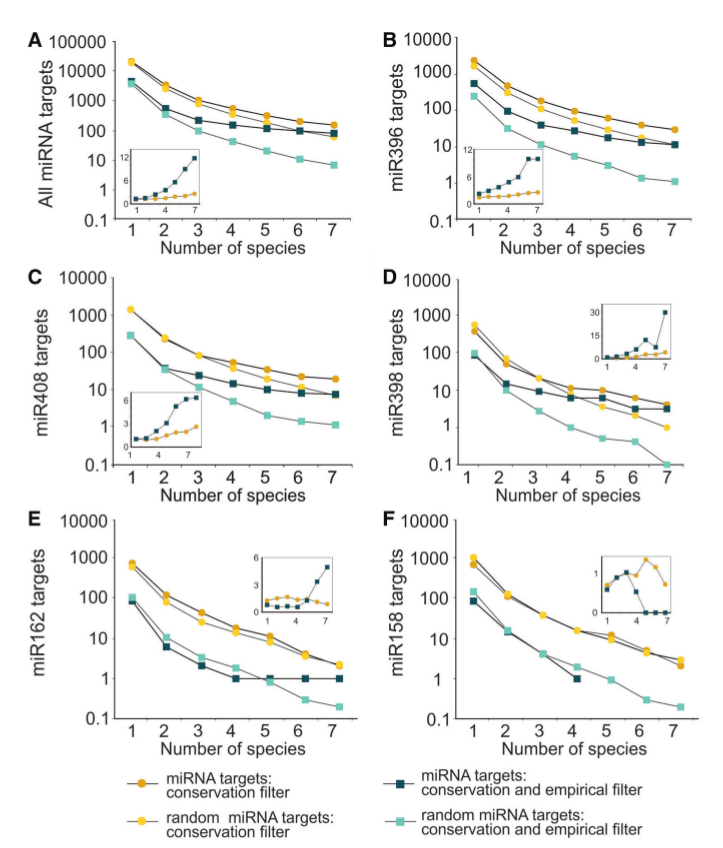
\includegraphics[width=0.9\textwidth]{NAR_fig2.png}
    \caption[Conservación de potenciales genes blanco en distintas especies]{Conservación de potenciales genes blanco en distintas especies. Todos los miARNs 
    \textbf{(A)}, miR396 \textbf{(B)}, miR408 \textbf{(C)}, miR398 \textbf{(D)}, miR162 \textbf{(E)}, miR158 \textbf{(F)}.
    Puntos naranja representan los genes blanco de miARNs usando filtro evolutivo.
    Puntos amarillos representan los genes blanco de las secuencias al azar usando filtro evolutivo.
    El cuadrado azul muestra los genes blanco de miARNs luego de aplicar filtros empíricos y evolutivos, mientras que el cuadrado celeste representa los genes blanco de las secuencias al azar en las mismas condiciones.
    Los recuadros muestran la relación señal/ruido.}
    \label{fig:NAR_fig2}
\end{figure}

\begin{figure}[htbp!] 
    \centering    
    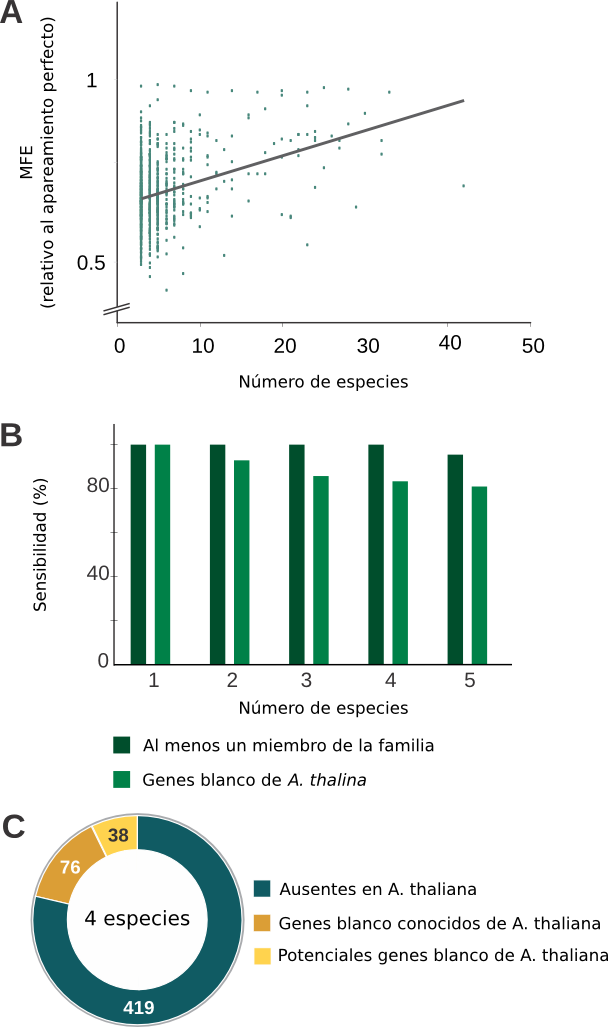
\includegraphics[width=0.6\textwidth]{NAR_fig3.png}
    \caption[Selección de genes blanco por conservación evolutiva de la secuencia]{Selección de genes blanco por conservación evolutiva de la secuencia.
    \textbf{(A)} Relación entre MFE y el número de especies en donde cada gen blanco fue detectado.
    \textbf{(B)} Sensibilidad de la estrategia, analizado de dos modos distinto. 
    Verde clarito: evaluando la presencia de genes validados en Arabidopsis y en verde oscuro teniendo en cuenta la presencia de por lo menos un gen blanco de cada familia regulada por miARNs.
    \textbf{(C)} Clasificación de los potenciales genes blanco presentes en al menos 4 especies.}
    \label{fig:NAR_fig3}
\end{figure}



\begin{landscape}
\begin{table}[]
\scriptsize
\centering
\caption{Detection of miRNA targets using different filters}
\label{table:NAR_table_2}
\begin{tabular}{lllllllllllllllll}
\multicolumn{1}{c}{} & \multicolumn{4}{c}{\textbf{Sin filtros}}                        & \multicolumn{4}{c}{\textbf{Filtros empíricos}}                  & \multicolumn{4}{c}{\textbf{Conservación 4 especies}}            & \multicolumn{4}{c}{\textbf{Todos los filtros}}                  \\
\multicolumn{1}{c}{} & \multicolumn{1}{c}{\textbf{miARN}} & \multicolumn{1}{c}{\textbf{scramble}} & \multicolumn{1}{c}{\textbf{}} & \multicolumn{1}{c}{\textbf{ratio}} & \multicolumn{1}{c}{\textbf{miARN}} & \multicolumn{1}{c}{\textbf{scramble}} & \multicolumn{1}{c}{\textbf{}} & \multicolumn{1}{c}{\textbf{ratio}} & \multicolumn{1}{c}{\textbf{miARN}} & \multicolumn{1}{c}{\textbf{scramble}} & \multicolumn{1}{c}{\textbf{}} & \multicolumn{1}{c}{\textbf{ratio}} & \multicolumn{1}{c}{\textbf{miARN}} & \multicolumn{1}{c}{\textbf{scramble}} & \multicolumn{1}{c}{\textbf{}} & \multicolumn{1}{c}{\textbf{ratio}} \\
\textbf{miR156}      & 3915           & 3994.4            & $\pm$ 149.9     & 1.0            & 890            & 704.7             & $\pm$  45.2      & 1.3            & 34             & 39.7              & $\pm$  3.1       & 0.9            & 10             & 5.4               & $\pm$  1.1       & 1.9            \\
\textbf{miR159}      & 1663           & 1283.7            & $\pm$  47.8      & 1.3            & 472            & 254.9             & $\pm$  21.9      & 1.9            & 20             & 10.1              & $\pm$  1.1       & 2.0            & 6              & 1.5               & $\pm$  0.5       & 4.0            \\
\textbf{miR160}      & 793            & 695.6             & $\pm$  30.5      & 1.1            & 277            & 157.5             & $\pm$  28.8      & 1.8            & 5              & 4.4               & $\pm$  0.9       & 1.1            & 4              & 0.5               & $\pm$  0.3       & 8.0            \\
\textbf{miR162}      & 1191           & 930.2             & $\pm$  139.5     & 1.3            & 108            & 164.7             & $\pm$  24.1      & 0.7            & 18             & 13.5              & $\pm$  3.5       & 1.3            & 1              & 1.8               &  $\pm$ 0.5       & 0.6            \\
\textbf{miR164}      & 2486           & 1480.2            & $\pm$  60.4      & 1.7            & 678            & 333.2             & $\pm$  32.2      & 2.0            & 39             & 12.4              & $\pm$  1.9       & 3.1            & 12             & 1.5               & $\pm$  0.5       & 8.0            \\
\textbf{miR166}      & 879            & 815.5             & $\pm$  45.0      & 1.1            & 231            & 129               & $\pm$  14.5      & 1.8            & 16             & 10.6              & $\pm$  1.4       & 1.5            & 6              & 0.9               & $\pm$  0.4       & 6.7            \\
\textbf{miR167}      & 1777           & 1364.2            & $\pm$  146.6     & 1.3            & 478            & 214.8             & $\pm$  27.5      & 2.2            & 22             & 20.2              & $\pm$  3.6       & 1.1            & 4              & 1.8               & $\pm$  0.5       & 2.2            \\
\textbf{miR168}      & 962            & 797.5             & $\pm$  48.5      & 1.2            & 209            & 185               & $\pm$  14.2      & 1.1            & 6              & 4.4               & $\pm$  0.8       & 1.4            & 1              & 1.1               & $\pm$  0.5       & 0.9            \\
\textbf{miR169}      & 1540           & 1047.2            & $\pm$  69.7      & 1.5            & 464            & 181.4             & $\pm$  15.6      & 2.6            & 26             & 11.1              & $\pm$  2.1       & 2.3            & 10             & 1.2               & $\pm$  0.2       & 8.3            \\
\textbf{miR171}      & 884            & 723.4             & $\pm$  32.1      & 1.2            & 202            & 113.8             & $\pm$  13.4      & 1.8            & 7              & 6.6               & $\pm$  1.4       & 1.1            & 2              & 0.7               & $\pm$  0.3       & 2.9            \\
\textbf{miR172}      & 3007           & 1693.7            & $\pm$  124.7     & 1.8            & 540            & 288.1             & $\pm$  40.3      & 1.9            & 34             & 17.7              & $\pm$  1.7       & 1.9            & 5              & 2.2               & $\pm$  0.6       & 2.3            \\
\textbf{miR319}      & 1363           & 1274.2            & $\pm$  113.6     & 1.1            & 324            & 249.2             & $\pm$  22.3      & 1.3            & 18             & 15                & $\pm$  2.8       & 1.2            & 7              & 1.8               & $\pm$  0.5       & 3.9            \\
\textbf{miR390}      & 873            & 814.4             & $\pm$  64.3      & 1.1            & 335            & 173               & $\pm$  22.5      & 1.9            & 8              & 4.7               & $\pm$  1.2       & 1.7            & 3              & 0.7               & $\pm$  0.5       & 4.3            \\
\textbf{miR393}      & 986            & 844.6             & $\pm$  58.7      & 1.2            & 276            & 124.6             & $\pm$  11.1      & 2.2            & 14             & 7.1               & $\pm$  1.2       & 2.0            & 5              & 0.5               & $\pm$  0.2       & 10.0           \\
\textbf{miR394}      & 1569           & 1531.4            & $\pm$  57.5      & 1.0            & 188            & 237.1             & $\pm$  25.0      & 0.8            & 26             & 21.4              & $\pm$  2.2       & 1.2            & 3              & 2.9               & $\pm$  0.5       & 1.0            \\
\textbf{miR395}      & 1472           & 1226.7            & $\pm$  66.7      & 1.2            & 426            & 217.6             & $\pm$  16.5      & 2.0            & 11             & 8.8               & $\pm$  1.3       & 1.3            & 6              & 1.3               & $\pm$  0.3       & 4.6            \\
\textbf{miR396}      & 4641           & 2979.3            & $\pm$  246.6     & 1.6            & 1246           & 390.5             & $\pm$  38.8      & 3.2            & 92             & 51.4              & $\pm$  5.9       & 1.8            & 26             & 5.4               & $\pm$  1.0       & 4.8            \\
\textbf{miR397}      & 1426           & 1050.9            & $\pm$  27.9      & 1.4            & 368            & 236.5             & $\pm$  23.5      & 1.6            & 26             & 9.7               & $\pm$  0.8       & 2.7            & 10             & 1.6               & $\pm$  0.3       & 6.3            \\
\textbf{miR398}      & 935            & 834               & $\pm$  34.5      & 1.1            & 376            & 144               & $\pm$  18.1      & 2.6            & 11             & 7.5               & $\pm$  1.6       & 1.5            & 6              & 1                 & $\pm$  0.3       & 6.0            \\
\textbf{miR399}      & 1192           & 1137.6            & $\pm$  72.0      & 1.0            & 275            & 207.8             & $\pm$  24.9      & 1.3            & 5              & 13.6              & $\pm$  1.7       & 0.4            & 1              & 1.5               & $\pm$  0.7       & 0.7            \\
\textbf{miR408}      & 2782           & 2502.9            & $\pm$  103.6     & 1.1            & 695            & 468.7             & $\pm$  50.8      & 1.5            & 51             & 35.1              & $\pm$  3.0       & 1.5            & 14             & 4.6               & $\pm$  0.8       & 3.0            \\
\textbf{miR827}      & 2261           & 2000.1            & $\pm$  119.8     & 1.1            & 317            & 297.1             & $\pm$  45.0      & 1.1            & 44             & 23.4              & $\pm$  3.9       & 1.9            & 4              & 2.3               & $\pm$  0.8       & 1.7            \\
\textbf{Total}       & 38597          & 31021.7           & $\pm$  1859.8    & 1.2            & 9375           & 5473.2            & $\pm$  576.3     & 1.7            & 533            & 348.4             & $\pm$  47.0      & 1.5            & 146            & 42.2              & $\pm$  11.3      & 3.5            \\
\textbf{Control}     &                &                   &                  &                &                &                   & $\pm$            &                &                &                   &                  &                &                &                   &                  &                \\
\textbf{miR158}      & 1364           & 1462.8            & $\pm$  69.1      & 0.9            & 170            & 208.7             & $\pm$  15.8      & 0.8            & 15             & 16                & $\pm$  1.7       & 0.9            & 1              & 1.9               & $\pm$  0.4       & 0.5            \\
\textbf{miR173}      & 1386           & 1232.1            & $\pm$  101.7     & 1.1            & 243            & 215.6             & $\pm$  23.4      & 1.1            & 11             & 12                & $\pm$  2.4       & 0.9            & 1              & 1.5               & $\pm$  0.4       & 0.7           \\
\multicolumn{17}{l}{a Sin filtros, búsqueda inicial utilizando los miARN consenso de 18nt y 3 mismatches.}\\
\multicolumn{17}{l}{b Filtros empíricos, energía de al menos 72\% del apareamiento perfecto y 1 mismatch en la posición 2-12 del par miARN-gen blanco.}\\
\multicolumn{17}{l}{c Conservación del ID tag en al menos cuatro especies.}\\
\multicolumn{17}{l}{d Todos los filtros, combinación de los filtros empíricos y de conservación en al menos cuatro especies.}\\
\multicolumn{17}{l}{e miARN, genes blanco para cada miARN específico.}\\
\multicolumn{17}{l}{f scramble, promedio de los genes blanco de 10 versiones al azar de cada miARN ± error estándar.}\\
\end{tabular}
\end{table}
\end{landscape}

\subsubsection{Identificación de nuevos genes blanco en \textit{A. thaliana} por conservación de la secuencia del gen blanco.}


Para encontrar nuevos genes blanco nos enfocamos en los genes potenciales que fueron seleccionados de nuestra estrategia utilizando solamente conservación evolutiva, debido a que los parámetros empíricos ya fueron utilizados extensamente en trabajos anteriores. \citep{Allen2005207,JonesRhoades2004787,Schwab2005517}.
En primer lugar, analizamos la detección de genes blanco validados previamente en \textit{A. thaliana} [basado en \citep{Fahlgren2010}] usando nuestra estrategia y encontramos que el 84\% de ellos estaban presentes en al menos 4 especies (Figura \ref{fig:NAR_fig3} B).
Consideramos esto como un buen resultado ya puede ser que no todos los genes blanco de Arabidopsis estén conservados evolutivamente.

Generalmente los miARNs en plantas regulan genes que codifican para proteínas de la misma familia, es por esto que evaluamos si por lo menos un miembro de cada familia era detectado en nuestro enfoque.
Encontramos genes blanco pertenecientes a casi todas las familias de genes codificantes para proteínas presentes en cuatro especies (Figura \ref{fig:NAR_fig3} B), con la excepción de TAS3, que es regulado por el miR390, al ser un ARN no codificante no es detectado por Blastx. 

Para encontrar nuevos genes blanco regulados por miARNs, nos enfocamos únicamente  en los potenciales genes blanco conservados en 4 especies, donde una de ellas es \textit{A. thaliana} (Figura 1, bin 1). 
Genes blanco de miARNs que no están presentes en \textit{A. thaliana} podrían incluir genes que perdieron su regulación durante la evolución o genes que hayan adquirido control por un miARN conservado más reciente en otras especies.
La conservación en cuatro especies fue elegida como un filtro evolutivo porque provee buena sensibilidad para genes blanco conocidos.

Identificamos 114 potenciales genes que satisfacen este criterio. Donde 76 de ellos son genes validados anteriormente o genes muy relacionados (Figura \ref{fig:NAR_fig3} C).
Curiosamente encontramos 38 genes que no tienen relación con genes blanco conocidos de miARNs y decidimos estudiar este grupo con mayor detalle.
Nos enfocamos primero en los genes que estaban presentes en un gran número de especies para tener mejor especificidad (Figura \ref{fig:NAR_fig2}) e intentamos validarlos utilizando 5' RACE PCR modificada \citep{Llave2002,Kasschau2003}.

Un potencial gen blanco del MiR408 era At5g21930 que codifica para P-TYPE ATPase OF ARABIDOPSIS 2 (PAA2) y estaba presente en 22 especies distintas incluido monocotiledóneas y dicotiledóneas.
MiR408 es inusual debido a que tiene un 5'-A, sin embargo >30\% de las secuencias maduro del miR408 corresponden a una variante corrida 1 nt que empieza con 5'-U \citep{Maunoury2011} (Figura \ref{fig:NAR_fig4} A).
La validación experimental reveló fragmentos de ARNm compatible con este último sitio de corte (Figura \ref{fig:NAR_fig4} A). 
PAA2 es necesaria para el transporte de iones de cobre a plastocianina \citep{Niyogi2005}, y su regulación por el miR408 está relacionada con el rol de este miARN en la homeostasis de cobre \citep{Yamasaki2007}.

Otro potencial candidato del miR408 era At3g22110 que codifica para PROTEASOME ALPHA SUBUNIT C1 (PAC1) y estaba presente en 20 especies. Por medio de 5' RACE PCR demostramos que este gen es gen blanco del miR408 (Figura \ref{fig:NAR_fig4} A). 
Curiosamente la interacción del par miARN-gen blanco tiene 3 mismatches en la región 5', y se hubiera perdido como potencial gen blanco si se aplicaban solamente los filtros empíricos.

Luego estudiamos los genes blanco del miR396, donde los genes SVP y SUI1 estaban presentes en 29 y 19 especies respectivamente.
Pero en ambos casos fallamos al obtener producto de la PCR utilizando 5' RACE PCR modificada.
La falta de regulación de este gen por el miR396 podría estar relacionado a la débil energía de hibridación del par miARN-gen blanco, aunque no podemos descartar que el miR396 esté controlando su traducción.

Otros dos potenciales genes blanco del miR396 eran At5g43060 y At3g14110 que codifican para la proteasa MMG4.7 y FLUORESCENT IN BLUE LIGTH (FLU), respectivamente.
Y en ambos casos pudimos detectar el corte (Figura \ref{fig:NAR_fig4} C y D).
%~ Ver
%~ Determination of MMG4.7 and FLU transcript levels in 35S:miR396 plants revealed a significant decrease of FLU and a minor effect on MMG4.7


En contraste con el miR408 y miR396, donde tienen varios potenciales genes blanco, obtuvimos un solo potencial gen blanco para el miR159, un factor de transcripción MYB que regula desarrollo del estambre y polen \citep{Millar2005}.
El otro potencial gen blanco era At4g27330, conocido como NOZZLE/SPOROCYTLESS.
Este factor de trascripción, que participa en desarrollo del estambre y óvulo \citep{Biology1999,Yang1999}, fue también validado por 5' RACE PCR (Figura \ref{fig:NAR_fig4} E).
%~ Ver
%~ In good agreement, 35S:miR159 caused a reduction of both MYB and NOZZLE transcript levels (Supplementary Figure S2). A miR159 target with a NOZZLE-like domain has been also recently validated in tomato (51), which together with our results point toward a general role of miR159 in the regulation of NOZZLE-like genes. 
Es interesante notar que al menos las funciones de NOZZLE y PAA2 pueden estar directamente relacionadas con el rol de genes blanco, ya descritos anteriormente, del miR159 y miR408 respectivamente.

PAA2, FLU y NOZZLE fueron detectados en mono y dicotiledóneas mientras que PAC1 y MMG4.7 fueron detectadas solamente en dicotiledóneas (Figura \ref{fig:NAR_fig4} A-E).
Las posiciones del sitio de unión del miARN-gen blanco están altamente conservadas y muchas de las posiciones variables corresponden a mismatches con el miARN o variaciones del tipo G-C/G-U.
Además este método no requiere que el sitio del gen blanco esté conservada, sino más bien que haya una interacción predicha con el miARN en distintas especies.
De esta manera el sitio de NOZZLE, donde la secuencia cambia en diferentes especies (Figura \ref{fig:NAR_fig4} E), pudo ser detectado por este enfoque.

\begin{figure}[htbp!] 
    \centering    
    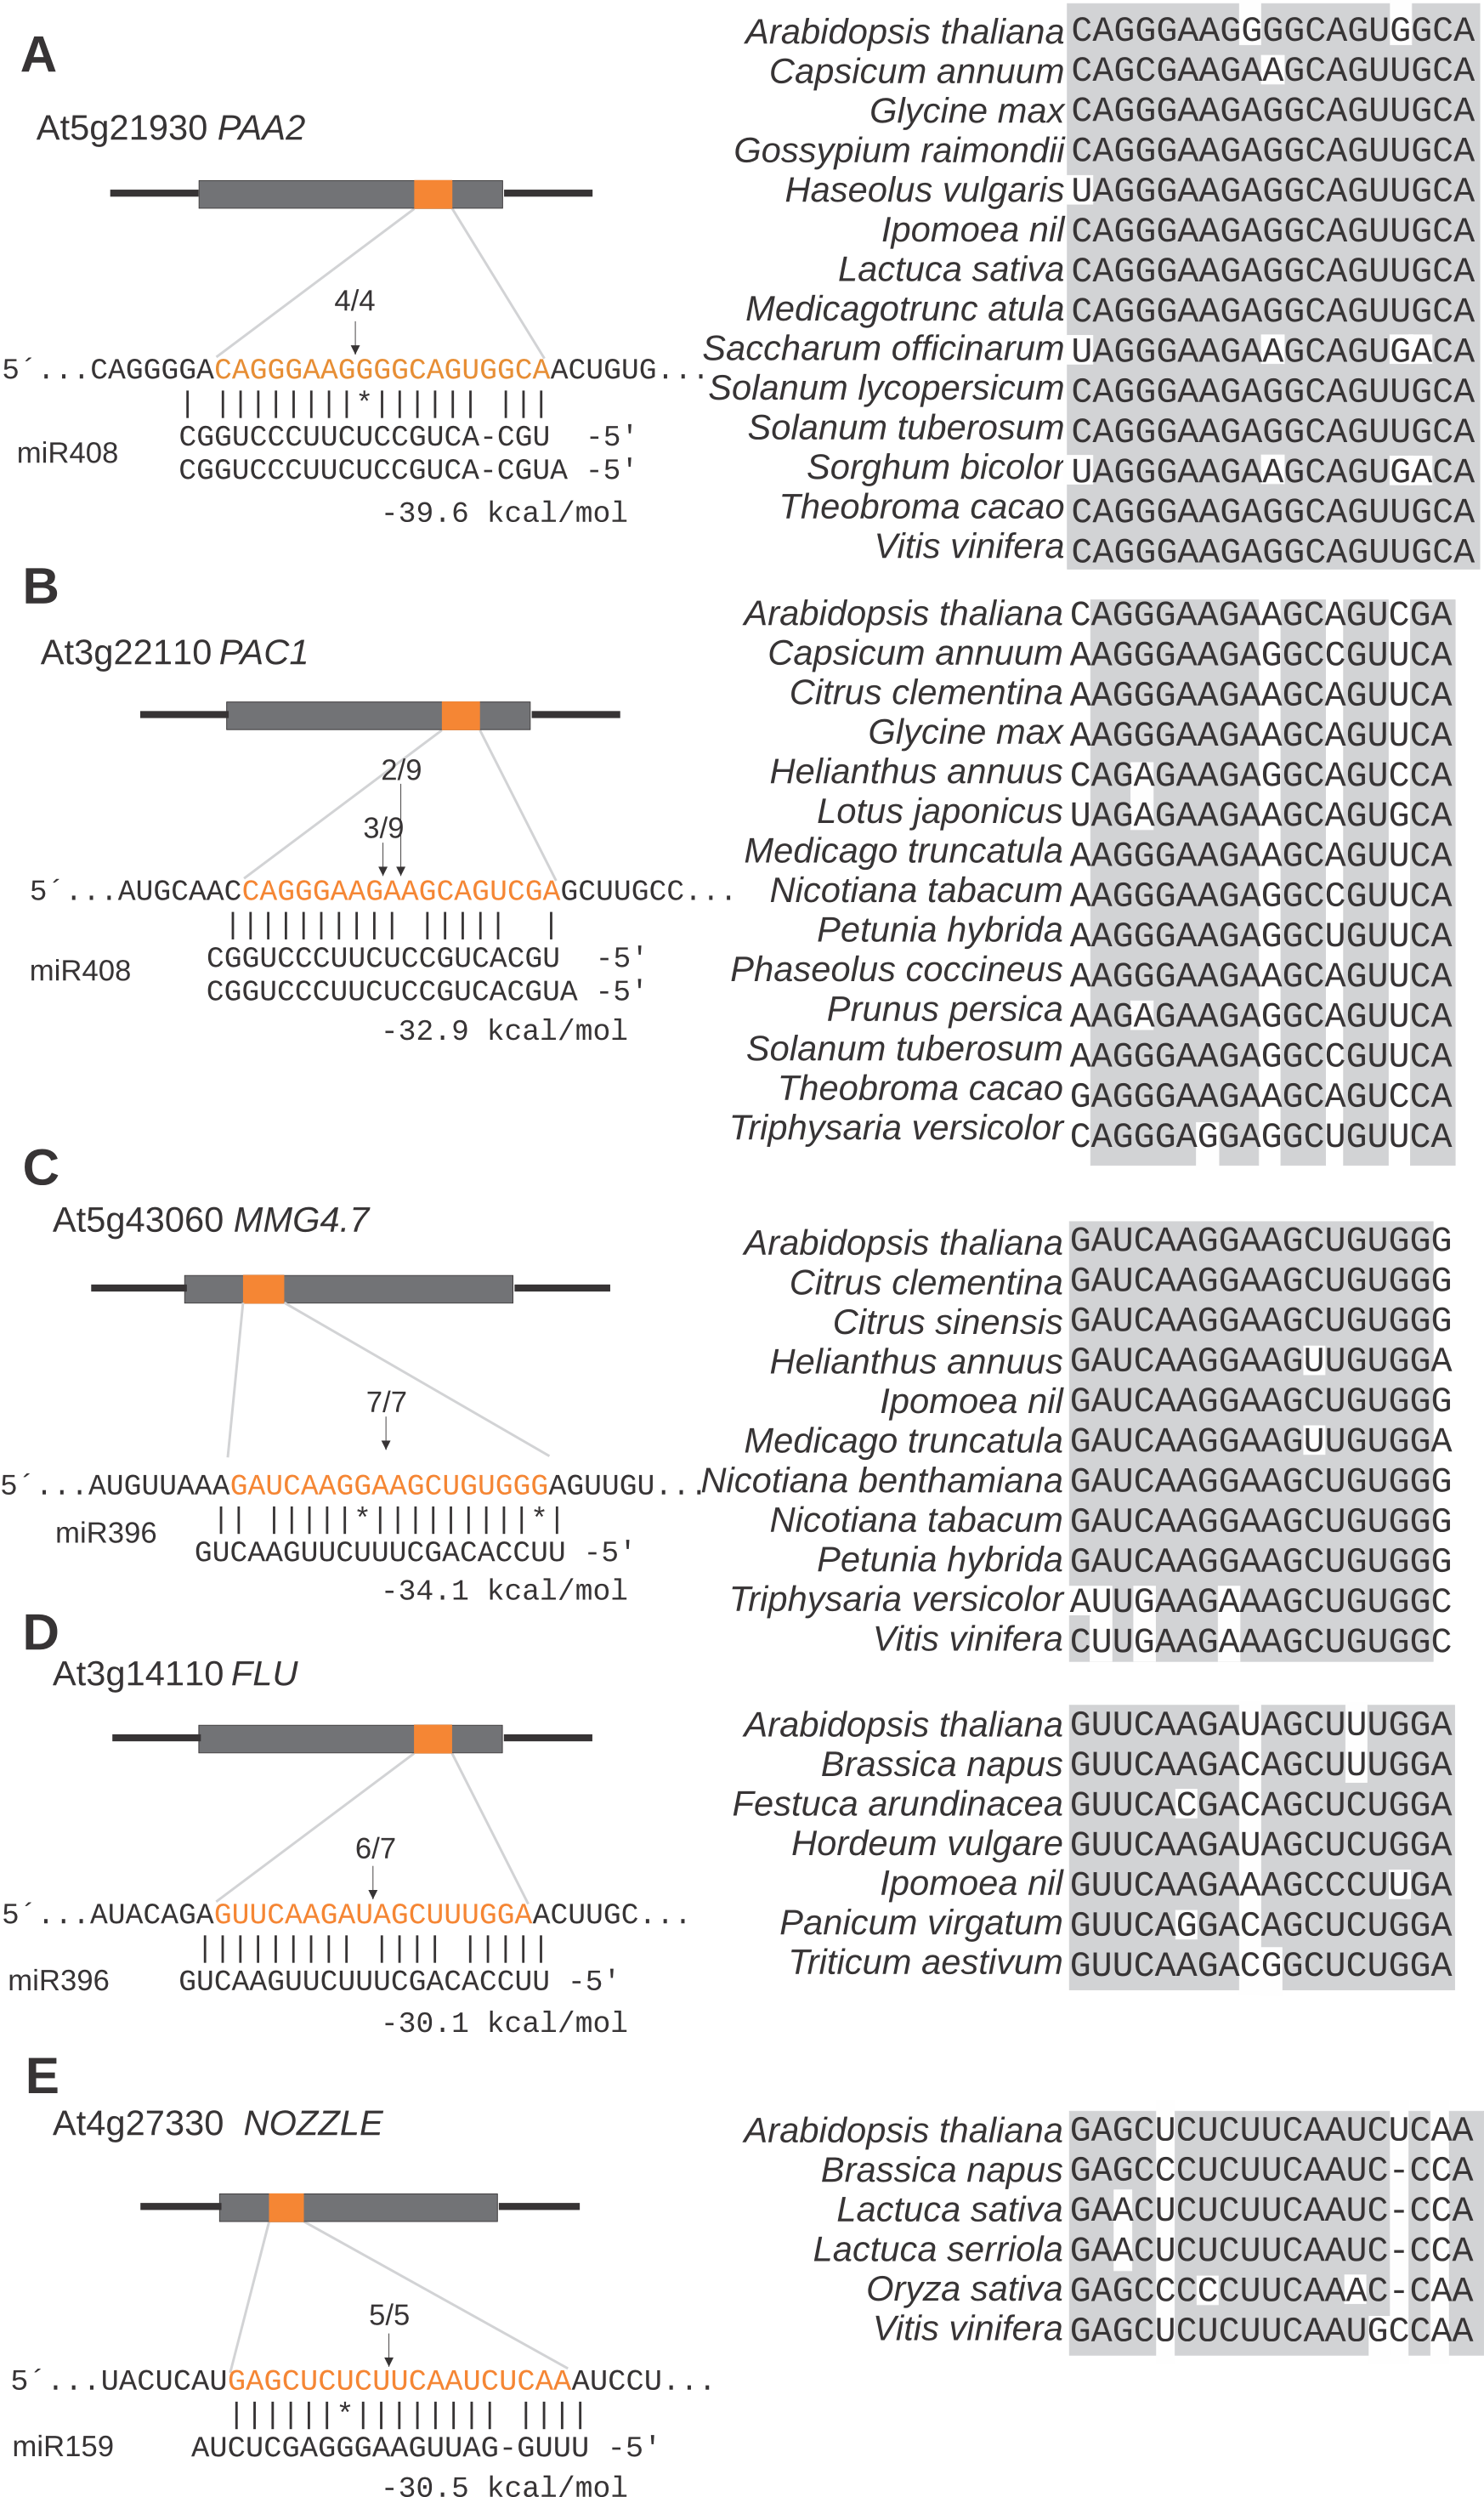
\includegraphics[width=0.7\textwidth]{NAR_fig4.png}
    \caption[Nuevos genes blanco validados en \textit{A. thaliana}.]{Nuevos genes blanco validados en \textit{A. thaliana}. 
    El alineamiento entre el miARN y los nuevos genes blanco identificados se muestran en la izquierda.
    La conservación evolutiva de la secuencia del sitio reconocido por el miARN en las especies seleccionadas se muestra a la derecha. La figura muestra las interacciones del miR408 con PAA2
    \textbf{(A)}, miR408 con PAC1 \textbf{(B)}, miR396 con MMG4.7 \textbf{(C)}, miR396 con FLU \textbf{(D)}, miR159 con NOZZLE \textbf{(E)}.
    Las flechas marcan el sitio de corte determinado por 5’RACE-PCR y los números indican la frecuencia de clonadao de cada fragmento.}
    \label{fig:NAR_fig4}
\end{figure}


\subsubsection{Identificación de nuevos genes blanco permitiendo interacciones G-U.}

Los genes blanco identificados utilizando la estrategia descrita anteriormente, tienen varios "mismatches" y "bulges" con sus miARNs, lo que puede ayudar a explicar por que se perdieron en trabajos anteriores. 
También notamos que muchas de estas nuevas interacciones miARN-gen blanco contenían posiciones que variaban alternadamente entre G-C y G-U en distintas especies.
Como consideramos G-U como "mismatch" en nuestra búsqueda inicial, decidimos realizar nuevamente la búsqueda con los miARNs consenso de 18nt pero permitiendo ahora 4 "mismatches", donde al menos uno de ellos tiene que ser del tipo G-U.
Esta búsqueda permitiría interacciones miARN-gen blanco con sólo 14 bases apareadas perfectamente.

Para compensar el uso de estos parámetros relajados en términos de "mismatches", requerimos que el gen blanco aparezca en al menos 10 especies distintas para aumentar la especificidad (Figura \ref{fig:NAR_fig5} A).
Encontramos 125 potenciales genes blanco en \textit{A. thaliana} teniendo en cuenta este criterio (Figura \ref{fig:NAR_fig5} A) y 34 de ellos no aparecían en las búsquedas anteriores.
El gen blanco CSD2 regulado por el miR398, que no apareció anteriormente, fue detectado con estos parámetros. 

Luego examinamos el último grupo de potenciales genes regulados por miARNs que estaban realizando funciones auxiliares a los genes blanco ya descritos para cada miARN. 
Y encontramos que el miR167 que regula factores de respuesta a auxina (ARFs), también regulaba potencialmente a un gen denominado IAA-ALANINE RESISTANT 3 (IAR3) (Figura \ref{fig:NAR_fig5} B y C), que está involucrado en el control de niveles libre de auxina \citep{Davies1999,Rampey2004}.

IAR3 en Arabidopsis tiene 3 "mismatches" con respecto al miR167, pero en la posición 12 de la interacción miARN-gen blanco, hay una interacción G-U en varias especies (Figura \ref{fig:NAR_fig5} B y C).
La técnica de 5’ RACE PCR confirmó que el gen realmente era gen blanco del miR167 (Figura \ref{fig:NAR_fig5} C).

\begin{figure}[htbp!] 
    \centering    
    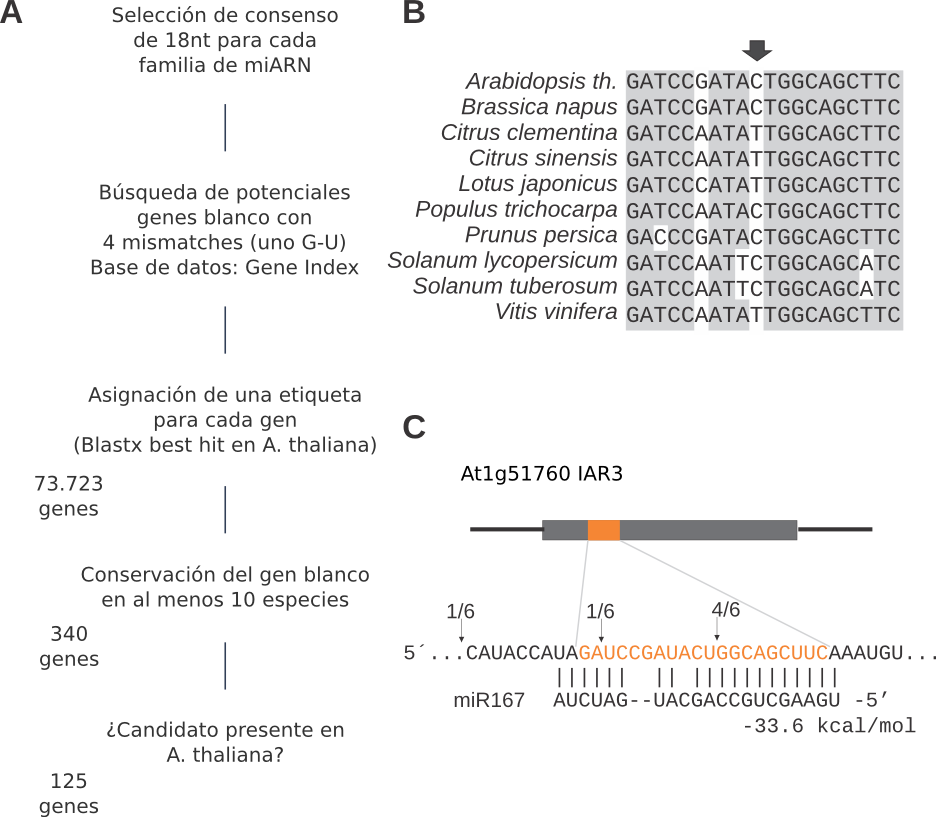
\includegraphics[width=0.8\textwidth]{NAR_fig5.png}
    \caption[Identificación de un nuevo gen blanco de miARN]{Identificación de un nuevo gen blanco de miARN, relajando los parámetros de interacción pero incrementando el parámetro de conservación evolutiva.
    \textbf{(A)} Esquema de la estrategia modificada para identificar genes blanco de miARNs.
    \textbf{(B)} Conservación del sitio blanco reconocido por el miARN en distintas especies.
    La flecha indica una variación de G-C o G-U con el miARN dependiendo de la especie.
    \textbf{(C)} Alineamiento en \textit{A. thaliana} del gen blanco IAR3 con el miR167. La flecha indica la posición del corte indicada por 5’RACE-PCR y el número indica la frecuencia de clonado de cada fragmento.}
    \label{fig:NAR_fig5}
\end{figure}


\subsubsection{Identificación de genes blanco específicos de \textit{Solanaceae}.}

Pensamos que la estrategia mostrada también se puede utilizar para encontrar genes blanco presentes específicamente en un grupo de especies relacionadas.
Por lo tanto intentamos demostrar esto, encontrando potenciales genes blanco específicos de la familia de \textit{Solanaceae}. 

Elegimos esta familia en particular, ya que 6 especies estaban bien representadas en la biblioteca utilizada.
La relación señal/ruido entre los genes blanco y las secuencias al azar era más de 2 cuando el filtro empírico o de conservación (en al menos 3 de las 6 especies \textit{Solanaceae} ) fueron aplicados (Figura \ref{fig:NAR_fig6} A).
Curiosamente, al aplicar ambos filtros dio como resultado una relación señal/ruido por encima de 6 (Figura \ref{fig:NAR_fig6} A), confirmando nuestros previos hallazgos de que ambos filtros mejoran la detección de genes blanco de miARNs.

Encontramos 132 potenciales genes blanco presentes en al menos 3 especies \textit{Solanaceae}. De este grupo, 41 genes no fueron detectados en otras especies (Figura 6B).
El gen blanco más común fue la metalotioneína MT2A, presente en las 6 \textit{Solanaceae}, como potencial gen blanco del miR398, mientras que MT2B, homólogo de este gen, fue detectado en 5 especies (Figura \ref{fig:NAR_fig6} B-D).

Luego, aprovechamos las plantas transgénicas de tabaco que contienen un transgén 35S.mir398 (A.F. Lodeyro, N. Carrillo y J.F. Palatnik resultados no publicados) y chequeamos la expresión de estos genes.
Encontramos que CSD2, un gen blanco conservado del miR398, disminuía su expresión > 10 veces en las plantas transgénicas 35S:miR398 comparadas con la planta salvaje (Figura \ref{fig:NAR_fig6} E).
Curiosamente, observamos que tanto MT2A como MT2B  disminuyeron sus niveles de transcripción > 5 veces en estas plantas (Figura \ref{fig:NAR_fig6} E).
Estos resultados concuerdan con la regulación de MT2A y MT2B por el miR398, aunque no necesariamente demuestra una interacción directa.
Además, estos resultados demuestran que los genes blanco presentes en un grupo específico de especies pueden ser encontrados utilizando esta estrategia.


\begin{figure}[htbp!] 
    \centering    
    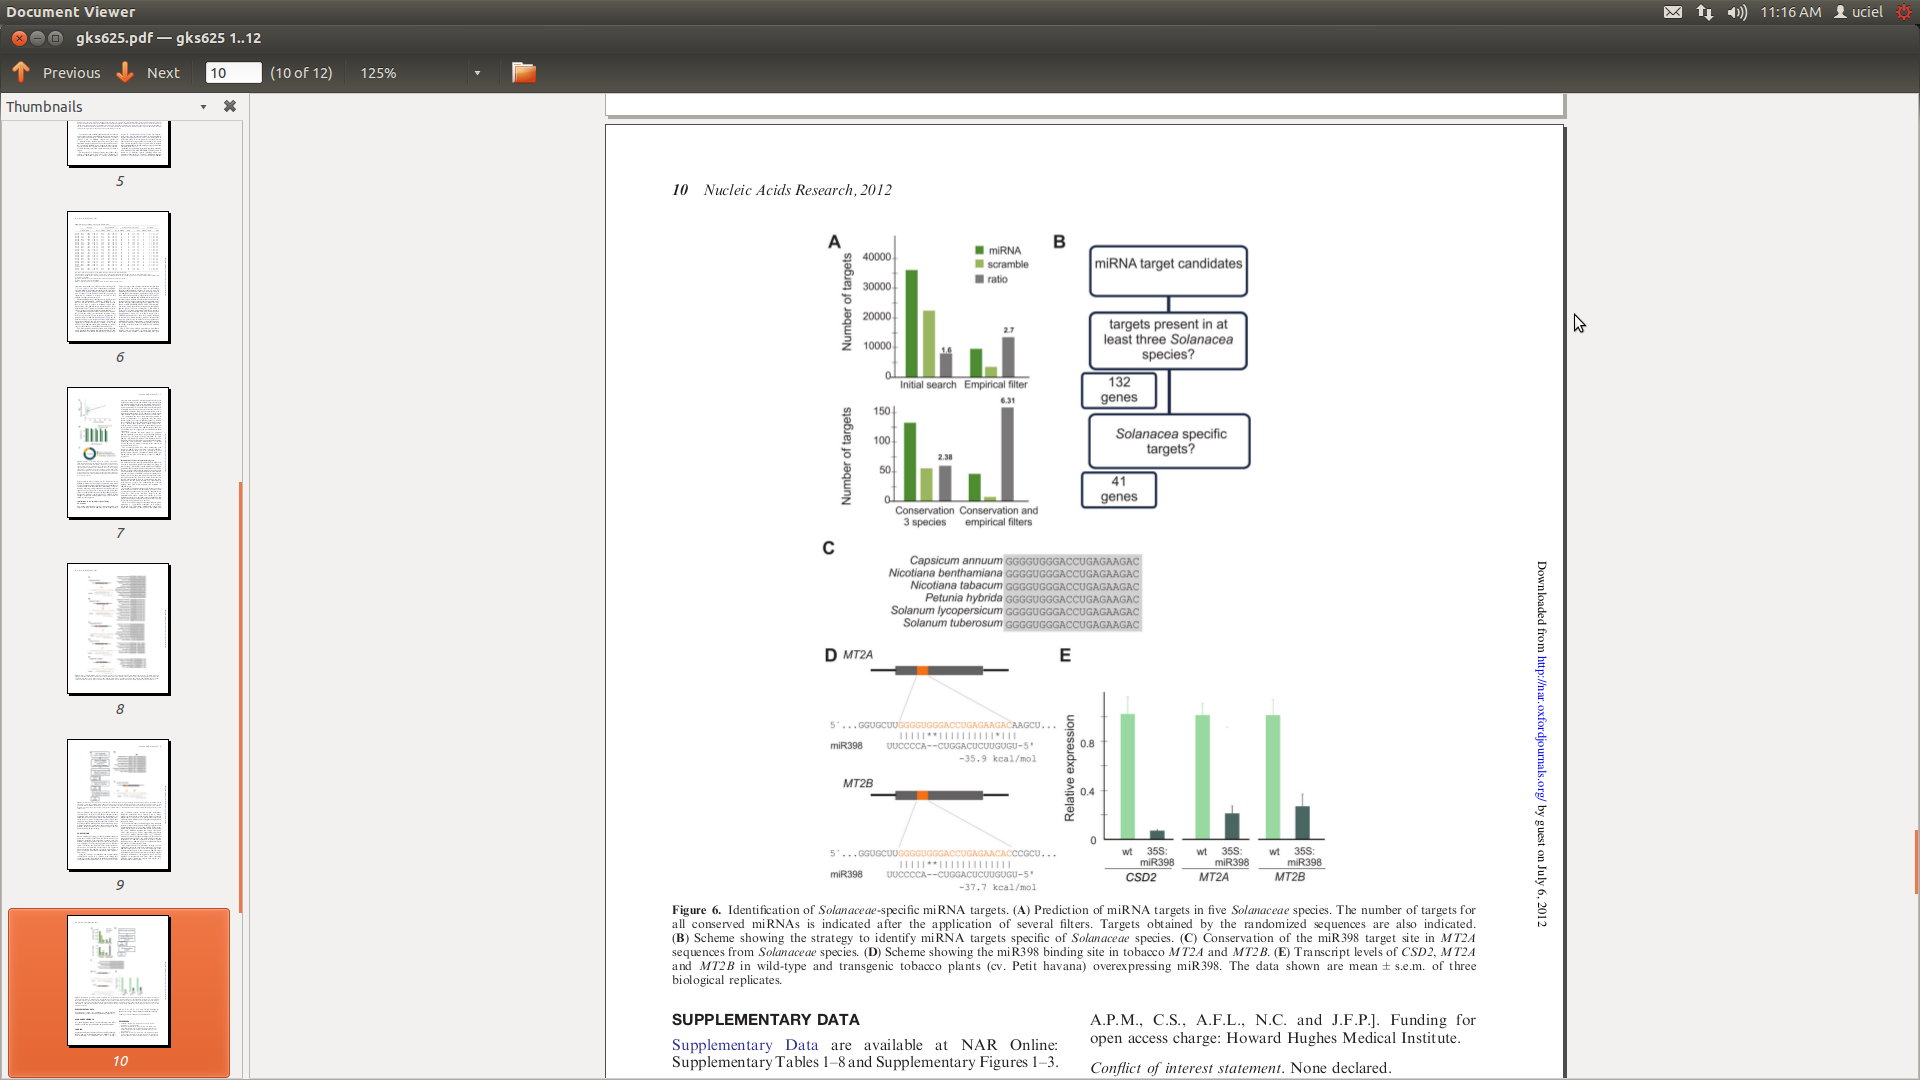
\includegraphics[width=0.7\textwidth]{NAR_fig6.png}
    \caption[Identificación de genes blanco de miARN, específicos de \textit{Solanaceae}]{Identificación de genes blanco de miARN, específicos de \textit{Solanaceae}.
    \textbf{(A)} Predicción de genes blanco de miARN en cinco especies de \textit{Solanaceae}.
    El número de genes blanco de todos los miARNs conservados juntos se muestra luego de aplicar distintos filtros.
    También se muestran los genes blanco obtenidos a partir de las secuencias al azar.
    \textbf{(B)} Esquema que muestra la estrategia para identificar genes blanco específicos de \textit{Solanaceae}.
    \textbf{(C)} Conservación del sitio reconocido por el mir398 con MT2A específico de \textit{Solanaceae}.
    \textbf{(D)} Esquema que muestra el sitio de unión entre el miR398 y MT2A y MT2B.
    \textbf{(E)} Niveles de transcriptos de CSD2, MT2A y MT2B en plantas salvajes y plantas transgénicas de tabaco (cv Petit havana) que sobreexpresan el miR398.  }
    \label{fig:NAR_fig6}
\end{figure}


\subsection{comTAR: una herramienta para la predicción de genes blanco regulados por miARNs en plantas.} 

A partir de la estrategia descrita en el capítulo anterior, que fue utilizada para encontrar y validar experimentalmente genes blanco regulados por miARNs en \textit{A. thaliana}, desarrollamos una herramienta web denominada comTAR\footnote{http://rnabiology.ibr-conicet.gov.ar/comtar} (Conserved plant miRNA target prediction tool) \citep{Chorostecki2014}.
La misma se puede utilizar para predecir potenciales genes blanco regulados por miARNs en plantas y está basada en la conservación evolutiva del par miARN-gen blanco con un número relajado de "mismatches".
ComTAR permite distintas opciones/parámetros de búsqueda que pueden ser modificados por el usuario:

\begin{itemize}
    \item Filtro de mismatch: Solamente un "mismatch" está permitido entre la posición 1 y la 11 de la secuencia del miARN consenso. (Sí/No).
    \item Corte por energía de hibridación: Se define que un gen blanco es predicho si la mínima energía de hibridación está por debajo del corte elegido.
    \item El número mínimo de especies donde un mismo TAG está presente para un miARN particular.
\end{itemize}

\subsubsection{Realizar la búsqueda de potenciales genes blanco de miARN}
Esta es la búsqueda por defecto.
El usuario puede realizar la búsqueda de genes blanco de miARNs conservados.
En la primer pantalla se muestra los potenciales genes blanco para un miARN dado (Figura \ref{fig:comTAR_find_targets}), con una breve descripción del gen, la familia a la que pertenece y además en cuantas y cuáles especies está presente.
También, para cada especie que está presente, se tiene acceso por pantalla al alineamiento del miARN-gen blanco, la energía de hibridación y los filtros empíricos de interacciones conocidas del par miARN-gen blanco (Figura \ref{fig:comTAR_fig2}).

\subsubsection{Realizar la búsqueda de familias de potenciales genes blanco de miARN}
Debido a que los miARNs en plantas en general regulan genes que codifican a proteínas de las misma familias, la herramienta tiene otra funcionalidad donde permite la búsqueda de genes agrupados por familias en vez de agruparlos por TAG.
De este modo genes en distintas especies con diferentes TAG, pero que pertenecen a la misma familia pueden ser detectados como familias de potenciales genes blanco.

\subsubsection{Realizar la búsqueda de un gen de interés para ver si es potencial gen blanco de algun miARN conservado}

El usuario puede introducir un locus TAG en particular (tanto de Arabidopsis como el 'gene ID' del Phytozome) y se identifica si este gen en particular puede ser un potencial gen blanco de algun miARN y en cuantas especies aparece.
En Arabidopsis se utiliza el LocusID como identificador, mientrás que en Phytozome este identificador varía según la especie y se puede ver la precedencia de cada especie en el sitio de Phytozome.

\subsubsection{Realizar la búsqueda de un miARN nuevo}
En esta parte del programa el usuario puede realizar la búsqueda de nuevos ARNs pequeños teniendo en cuenta que la secuencia introducida tiene que ser de 18nt de largo (posiciones 2-19).
Luego de la búsqueda, se da un link al usuario y después de unas horas, cuando haya sido procesado el cálculo, el usuario puede entrar a ese link y navegar los resultados por pantalla.



\begin{figure}[htbp!] 
    \centering    
    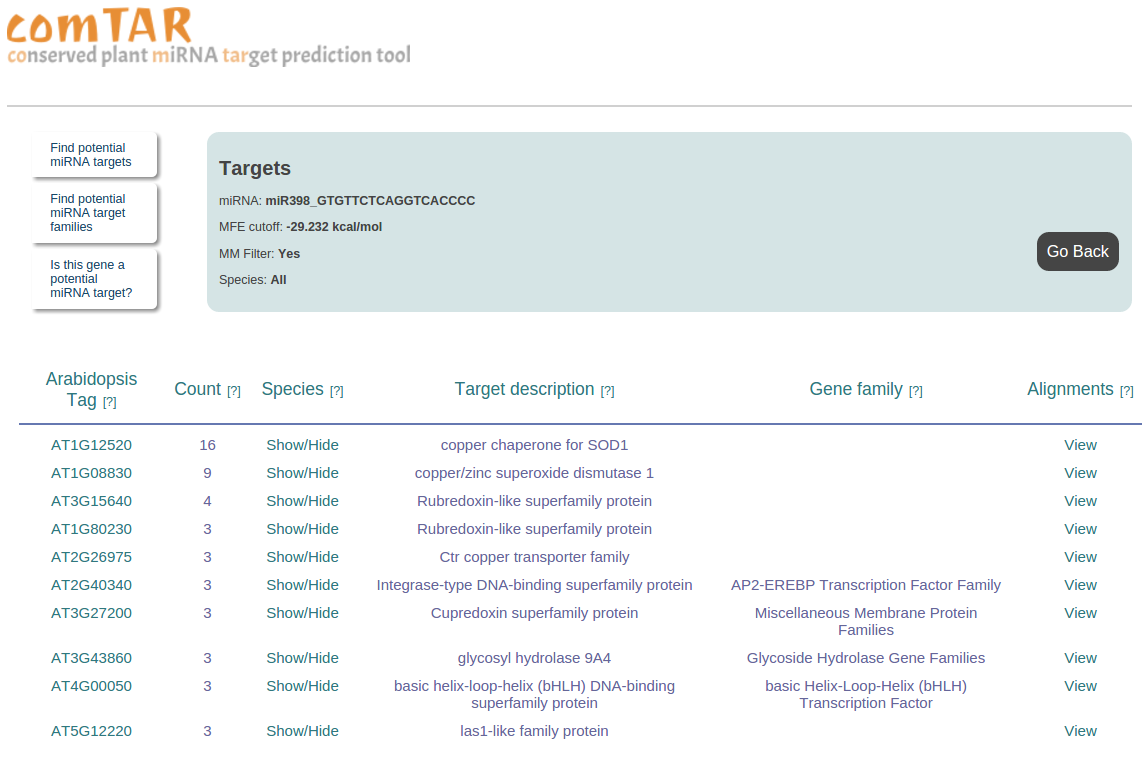
\includegraphics[width=1\textwidth]{comTAR_find_targets.png}
    \caption[Resultados del comTAR para el miR398]{Resultados de la búsqueda de comTAR, con parámetros por defecto para el miR398}
    \label{fig:comTAR_find_targets}
\end{figure}


\begin{figure}[htbp!] 
    \centering    
    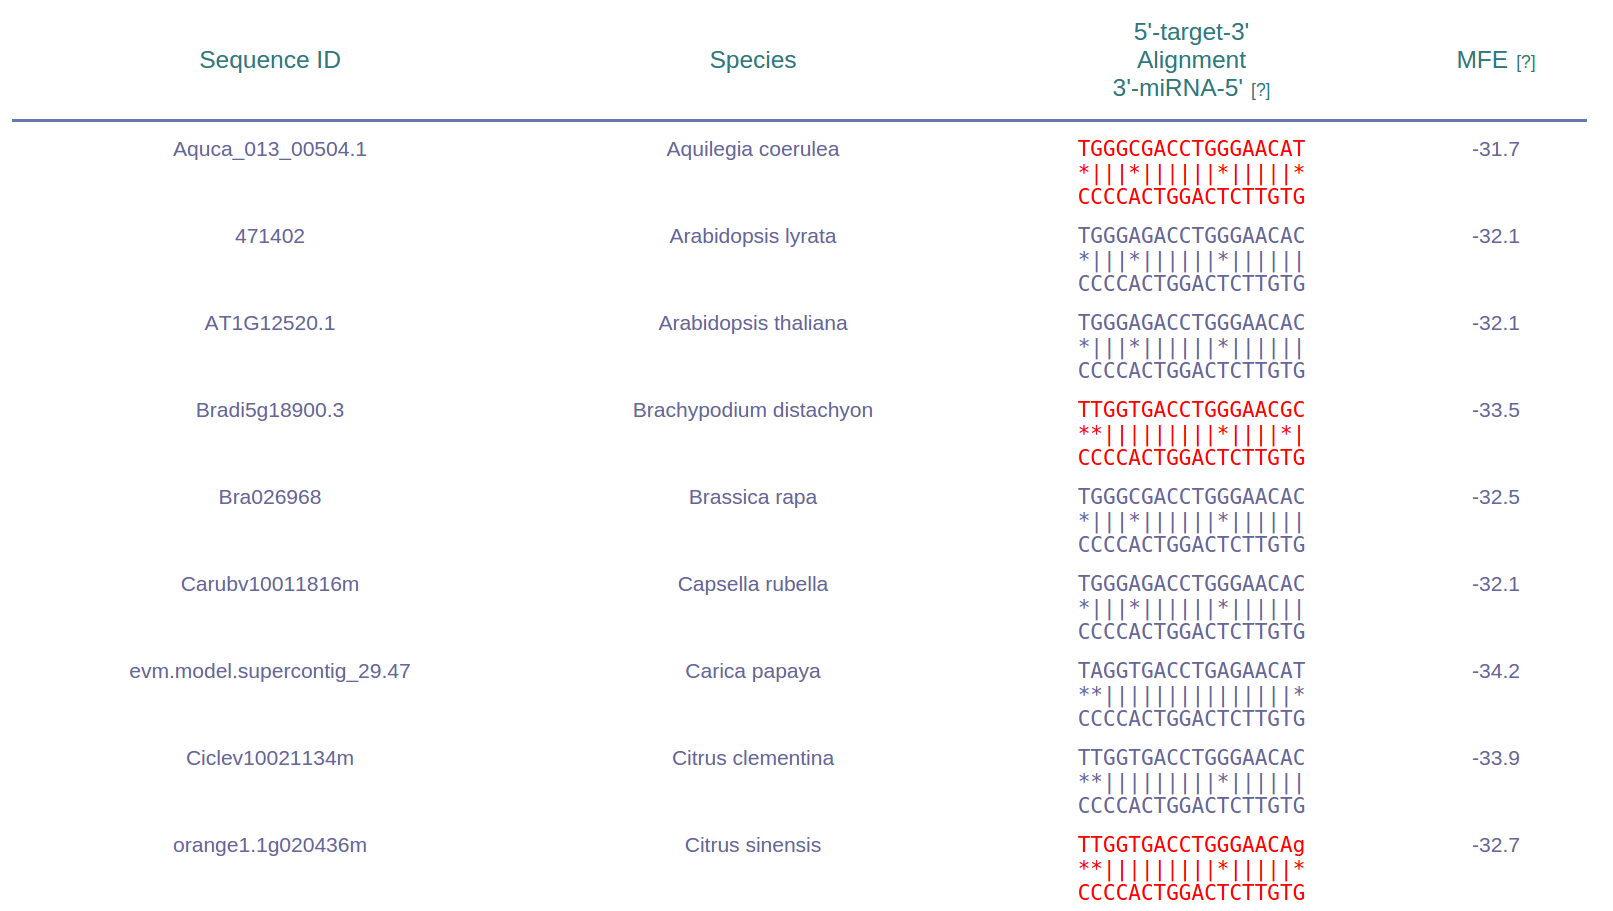
\includegraphics[width=1.1\textwidth]{comTAR_fig2.png}
    \caption[Salida del comTAR]{Parte de la salida de comTAR mostrando el par miR398/SOD1 (At1g12520) en diferentes especies}
    \label{fig:comTAR_fig2}
\end{figure}



%*******************************************************************************
%****************************** Second Chapter *********************************
%*******************************************************************************
\graphicspath{{Chapter2/Figs/}}

\setcounter{chapter}{5}
\chapter*{Resultados y Discusión Capítulo 2} 
\addcontentsline{toc}{chapter}{Resultados y Discusión Capítulo 2}

{\LARGE Estudios genómicos sobre la biogénesis de precursores de miARN en plantas}


\section{Introducción}
Los miARNs son una clase de ARNs de 20-22nt de largo que son originados de genes endógenos y regulan otros ARNs por complementariedad de bases \citep{Voinnet2009669}.
Se distinguen de otros ARNs pequeños por su biogénesis única que involucra el corte preciso del precursor, para liberar el miARN maduro.
Aunque la evidencia actual indica que los miARNs han surgido y especializada de forma independiente en animales y las plantas, su biogénesis depende del reconocimiento de claves estructurales ubicadas en los precursores de miARN \citep{pmid21554756,citeulike:8816489,Bologna11112012}.

En nuestro grupo actualmente se está estudiando la biogenesis de miARNs, específicamente como los precursores son reconocidos y procesados en plantas \citep{Bologna2013}.
Estos precursores tienen una estructura de tallo-burbuja característica \citep{Jones-Rhoades2006}, que se cree que proporciona las claves para el procesamiento del mismo y la liberación de los ARN pequeños de 21 nt.

Mientras que los precursores de miARN en animales tienen estructuras homogéneas, los precursores de miARNs en plantas constituyen una amplia gama de estructuras, y sus longitud pueden variar entre 50 y 900 nucleótidos \citep{Bologna2013,citeulike:8816489}.
Esa variabilidad se da entre distintas familias de precursores, pero a veces también entre una misma familia de precursores en distintas especies (Figura \ref{fig:hairpin_distribution}).

Además, en las plantas, las mutaciones que impiden la biogénesis o actividad de los miARNs, tales como \textit{hyl1}, \textit{hen1} y \textit{ago1}, conducen al aumento en los niveles de los transcriptos de muchos de los genes blanco de miARNs (aproximadamente un 45\% de todos los blancos) \citep{Han2004,pmid12747833,pmid16889646,Allen2005207}.
Esto sugiere que el mecanismo que involucra el corte y degradación de los ARNm es un componente importante de la represión inducida por los miARNs en plantas \citep{Jones-Rhoades2006, Voinnet2009669}.

\begin{figure}[htbp!] 
    \centering    
    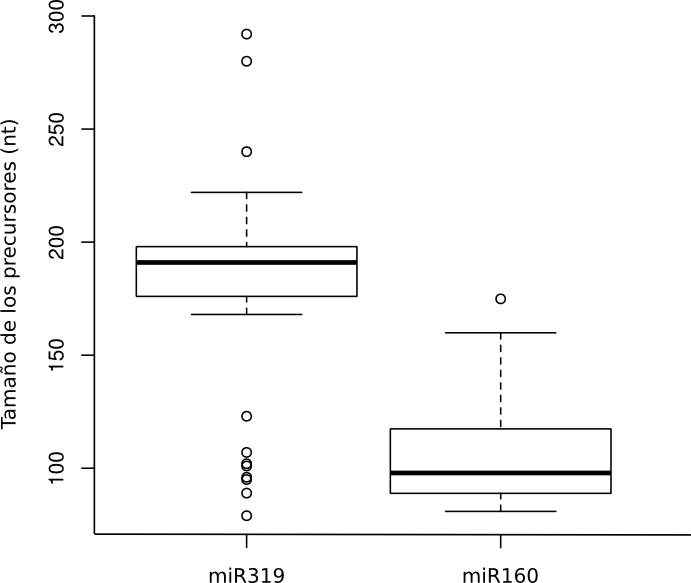
\includegraphics[width=.7\textwidth]{hairpin_distribution.png}
    \caption[Tamaño de precursores]{Tamaño de precursores. Se muestra el tamaño (nt) de dos familias de precursores en distintas especies.}
    \label{fig:hairpin_distribution}
\end{figure}

En particular, la biogénesis de los miARNs es un proceso clave porque determina la secuencia exacta de nucleótidos del ARN pequeño funcional.
Si bien en el caso de animales está claro cuáles elementos estructurales son reconocidos en los precursores durante su procesamiento, poco se sabía sobre el reconocimiento de los precursores de plantas por la maquinaria de procesamiento.

Muchos precursores en plantas tienen un tallo de $\sim$15 nt debajo del duplex miARN/miARN* seguido por un loop interno, que sirve como una señal estructural de reconocimiento por la maquinaria de procesamiento \citep{pmid17369351,pmid16751099,Mateos2010,pmid20015654}.
Sin embargo, este determinante de procesamiento no se encuentra en todos los precursores \citep{Mateos2010}.
Además, la biogénesis de los miARNs conservados evolutivamente como ser el miR319 y miR159 comienzan con un corte al lado del loop interno y continúa con 3 cortes adicionales en una dirección de burbuja a base hasta que finalmente el miARN es liberado \citep{Bologna2013,pmid19850910}.
Se ha demostrado que otros precursores de plantas liberan otros ARNs pequeños además del miARN \citep{pmid15314213,pmid20696037}, aunque los mecanismos de procesamiento subyacentes eran desconocidos.

\section{Resultados y Discusión}

%~ ################################################# 
%~ Procesamiento de precursores de miARNs en plantas
%~ #################################################

\subsection{Procesamiento de precursores de miARNs en plantas}
\label{sec:procesamiento}

En esta parte del proyecto de tesis y en el marco de una colaboración con el grupo del Dr. Blake Meyers (Delaware,USA), el cual se especializa en secuenciación y análisis de ARN pequeños, nos propusimos entender cómo se procesan los precursores de miARNs plantas. 
Colegas del laboratorio realizaron una estrategia para analizar sistemáticamente intermediarios de procesamiento de miARNs y caracterizar la biogénesis de la mayoría de los miARNs conservados presentes en \textit{A. thaliana} mediante técnicas de secuenciación de alto rendimiento, utilizando los equipos de última generación disponibles en Delaware (USA).
Esta técnica desarrollada en el laboratorio se conoce como SPARE \citep{Schapire2013} (del inglés Specific Parallel Amplification of RNA Ends).
Utilizando esta técnica encontramos que los miARNs son procesados por cuatro mecanismos, dependientes de la dirección secuencial de la maquinaria de procesamiento y del número de cortes requeridos para liberar el miARN.
La clasificación de los precursores, teniendo en cuenta los mecanismos de procesamiento, reveló determinantes estructurales específicos para cada grupo.
Se encontró que la complejidad de las vías de procesamiento de miARN se produce tanto en precursores jóvenes como en conservados y que los miembros de la misma familia pueden ser procesados de diferentes maneras.
Además hemos observado que diferentes determinantes estructurales compiten por la maquinaria de procesamiento y que miARNs alternativos pueden ser generados a partir de un único precursor.
Los resultados ofrecen una explicación para la diversidad estructural de los genes de precursores de miARN en plantas y nuevas perspectivas hacia la comprensión de la biogénesis de los ARNs pequeños \citep{Bologna2013}.


\subsubsection{Análisis de datos y precursores detectados}
Mediante la cantidad de cortes detectados la técnica de SPARE permite definir si el mecanismo es base a loop o loop a base.
Esta técnica arroja una gran cantidad de datos producto de la secuenciación de alto rendimiento, por lo que se necesita de un enfoque bioinformático para la interpretación de los resultados.
Por la gran cantidad de precursores a estudiar y el número de bibliotecas se necesitó un análisis previo de los datos y una forma de presentarlos.
Para esto construimos e implementamos un pipeline bioinformático utilizando "in-house" scripts y datos disponibles de miRBASE para poder analizar los datos de las bibliotecas de deep-sequencing obtenidos a partir de la técnica de SPARE.

Un precursor fue considerado como detectado si más de tres lecturas corresponden a la secuencia de ese precursor.
De esta manera encontramos fragmentos de ARN que corresponden a 129 precursores, 71 de ellos de miARNs conservados y 58 de miARNs jóvenes (Figura \ref{fig:GR_fig1C}).
Mediante el análisis de los datos arrojados de la estrategia bioinformática pudimos definir la dirección de procesamiento de la mayoría de los precursores en \textit{A. thaliana}.
De los cuales 32 de ellos fueron definidos como procesados por un mecanismo de base a loop, ya que se encontraron los cortes en la parte proximal del duplex miARN/miARN* sin detectar cortes en la parte de arriba del duplex, como en el caso del miR168a, miR172b y el miR395b (Figura \ref{fig:GR_fig2A}).
Además encontramos 16 precursores de miARNs conservados con cortes detectados (>5\%) en el lado distal del miARN/miARN* los cuales fueron definidos como loop a base (Figura \ref{fig:GR_fig4A}).

\begin{figure}[htbp!] 
    \centering    
    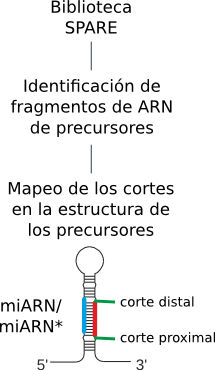
\includegraphics[width=.5\textwidth]{GR_fig1C.png}
    \caption[Esquema del procedimiento para analizar los datos de SPARE]{Esquema del procedimiento para analizar los datos de SPARE.}
    \label{fig:GR_fig1C}
\end{figure}

\begin{figure}[htbp!] 
    \centering    
    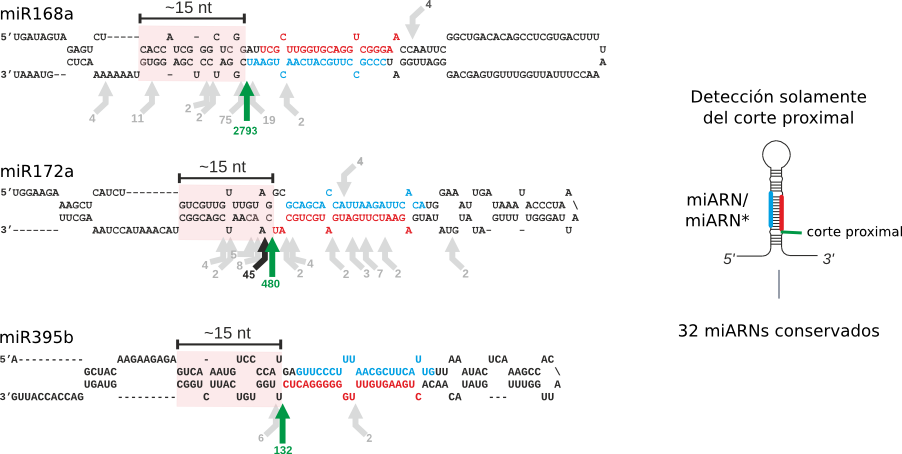
\includegraphics[width=1\textwidth]{GR_fig2A.png}
    \caption[Identificación y caracterización de precursores de miARNs procesados de base a loop]{Identificación y caracterización de precursores de miARNs procesados de base a loop.
            Esquema donde se muestra la estructura secundaria del miR168a, miR172b y miR395b.
            Las flechas indican la posición y número de lecturas de los cortes del precursor identificado.
            Flechas en verde muestra el corte más abundante, que también coincide con al corte proximal del miARN/miARN*.
            Flechas en negro muestran otros cortes con al menos 5\% de abundancia del número total de cortes, mientras que otros cortes minoritarios se muestran con una flecha gris.
            Con rosa se resalta el stem de 15nt debajo del corte proximal.
            El miARN se indica en color rojo y el miARN* en color azul.
            La imagen de la derecha muestra el patrón de corte típico detectado en la biblioteca de SPARE para estos precursores.}
    \label{fig:GR_fig2A}
\end{figure}


\begin{figure}[htbp!] 
    \centering    
    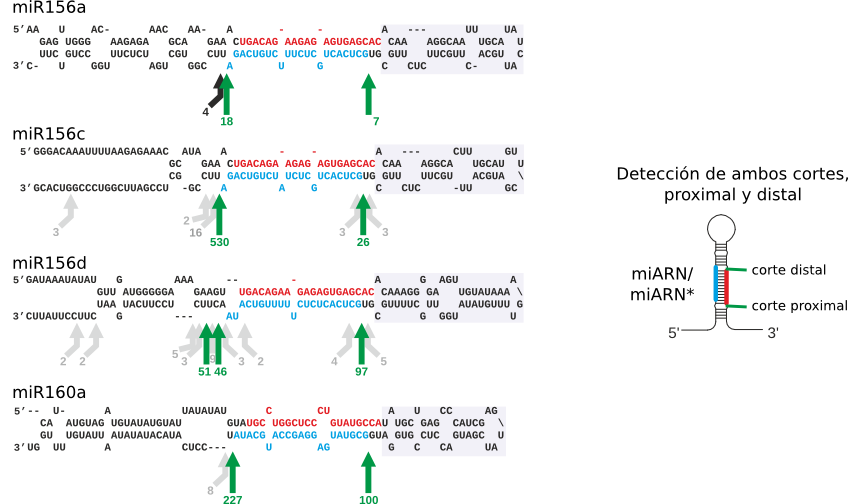
\includegraphics[width=1\textwidth]{GR_fig4A.png}
    \caption[Identificación y caracterización de precursores de miARNs procesados de loop a base]{Identificación y caracterización de precursores de miARNs procesados de loop a base. 
    Esquema donde se muestra la estructura secundaria del miR156a, miR156c, miR156d y miR160a.
    Las flechas indican la posición y número de lecturas de los cortes del precursor identificado.
    Flechas en verde muestra el corte más abundante, que también coincide con al corte proximal del miARN/miARN*.
    Flechas en negro muestran otros cortes con al menos 5\% de abundancia del número total de cortes, mientras que otros cortes minoritarios se muestran con una flecha gris.
    Con gris se resalta el stem de arriba del miR156 y miR160. El miARN se indica en color rojo y el miARN* en color azul.
    La imagen de la derecha muestra el patrón de corte típico detectado en la biblioteca de SPARE para estos precursores.
}
    \label{fig:GR_fig4A}
\end{figure}

\subsubsection{Estructura secundaria de los precursores}
Para ver si había diferencias estructurales para los precursores con diferentes mecanismos de procesamiento, determinamos la estructura secundaria de precursores detectados que se procesan en dirección base a loop (Figura \ref{fig:GR_fig2C}) y los que se procesan loop a base (Figura \ref{fig:GR_fig4C}).
Obtuvimos las estructuras secundarias para cada precursor.
Definimos a una coincidencia en cada posición con un 0, mientras que "bulges" y "mismatches" los consideramos como 1.
El lado proximal del duplex miARN/miARN* fue definido como la posición +1 y analizamos desde la posición -25 a la posición +40 (Figura \ref{fig:GR_fig2C} y \ref{fig:GR_fig4C}). 

\subsubsection{Procesamiento de base a loop}

Consideramos la estructura secundaria de 32 precursores analizados en esta parte del trabajo que se procesan de base a loop y todos ellos tienen un claro tallo inferior de 15 nt de largo (Figura \ref{fig:GR_fig2C}).
Además este tallo se pudo ver tanto para los precursores validados experimentalmente que se procesan de base a loop como para todos los precursores conservados (Figura \ref{fig:GR_fig2C} en violeta).
Pero pudimos observar que las bases inmediatamente debajo del duplex miARN/miARN* (posición -2 y -1) tienden a estar desapareadas (Figura \ref{fig:GR_fig2C}).
Además las posiciones -3 y -4 y las 3 últimas posiciones del stem inferior (-13,-14 y -15) están apareadas casi siempre (Figura \ref{fig:GR_fig2C}).
En general, nuestros resultados muestran que los precursores procesados en una dirección base a loop son más uniformes de lo que se pensaba previamente y que al menos algunos de los precursores no detectados como base a loop probablemente tengan otros determinantes específicos de ARN.

\subsubsection{Procesamiento de loop a base}
Estos precursores, que tienen un procesamiento loop a base, tienen un corte mayoritario que se puede detectar en nuestras bibliotecas.
Este corte es el esperado en la dirección de procesamiento de precursores con un mecanismo de loop a base.
Con la excepción de dos miARNs (miR396a y miR162b) estos precursores no tienen una estructura obvia debajo del duplex miARN/miARN* (Figura \ref{fig:GR_fig4C}).
Estos precursores tienen una región terminal estructurada (Figura \ref{fig:GR_fig4C}), que tiene un tamaño homogéneo de ~42nt que incluye un loop corto en contraste con la misma región en los precursores que se procesan de base a loop donde es más variable (Figura \ref{fig:GR_fig2C} y \ref{fig:GR_fig4C}). 

En esta segunda parte del proyecto de tesis presentamos un estrategia y realizamos un análisis sistemático para la identificación de la biogénesis de precursores de miARNs desde un punto de vista genómico.
De esta manera pudimos encontrar la dirección de procesamiento de la mayoría de los precursores de miARNs en \textit{A. thaliana}.

\begin{figure}[htbp!] 
    \centering    
    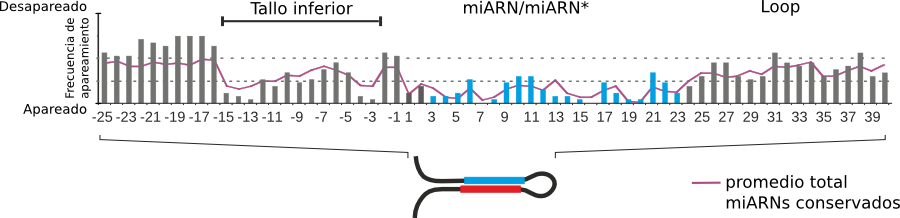
\includegraphics[width=1\textwidth]{GR_fig2C.png}
    \caption[Estructura secundaria de precursores de base a loop]{Estructura secundaria de precursores detectados que se procesan en dirección base a loop.
    Los matches en cada posición los consideramos como 0, mientras que "bulges" y "mismatches" fueron considerados como 1.
    La estructura secundaria considerando todos los miARNs conservados se indica con color violeta.
    }
    \label{fig:GR_fig2C}
\end{figure}

\begin{figure}[htbp!] 
    \centering    
    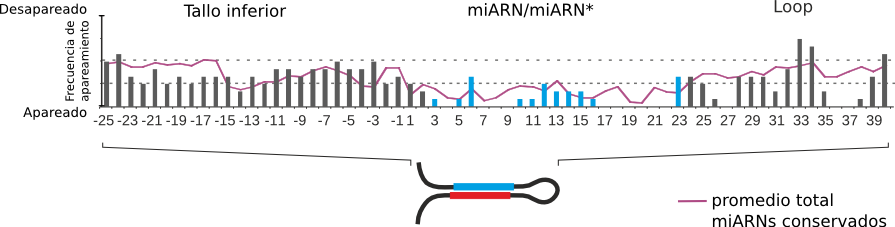
\includegraphics[width=1\textwidth]{GR_fig4C.png}
    \caption[Estructura secundaria de precursores de loop a base]{
    Estructura secundaria de precursores detectados que se procesan en dirección loop a base.
    Los matches en cada posición los consideramos como 0, mientras que "bulges" y "mismatches" fueron considerados como 1.}
    \label{fig:GR_fig4C}
\end{figure}


Estos resultados fueron publicado en la revista Genome Research \citep{Bologna2013}.
Em este mismo artículo se pudo demostrar que los precursores de miARNs en plantas, se pueden agrupar por cuatro mecanismos de procesamiento con distintas características (Figura \ref{fig:mecanismos}).

\begin{itemize}
    \item En los precursores con un mecanismo \textbf{corto de base a loop}, un loop interno seguido por un tallo inferior de $\sim$15nt especifica la posición del primer corte.
        Esta estructura se encuentra en la mayoría de familias de miARNs \citep{Mateos2010,pmid20015653,pmid20015654}.
        A pesar de que el tallo puede contener bulges, la transición de un loop interno (simple hebra) al tallo inferior es bastante marcada, y tres pares de bases apareadas generalmente definen el comienzo del tallo inferior del precursor \citep{Bologna2013}.
        El segundo corte procede a una distancia fija de $\sim$21 nt desde la posición del primer corte.
    \item En los precursores con un mecanismo \textbf{secuencial de base a loop} (ej: familia del miR169), el primer corte procede como en los cortos de base a loop, pero luego son necesario dos cortes más para liberar el miARN, generando en el proceso niveles bajos de RNA pequeños adicionales \citep{Bologna2013}.
    \item En los precursores con un mecanismo \textbf{cortos de loop a base} (ej: familia del miR156 y miR160), el procesamiento es guiado por un tallo superior, y son necesarios dos cortes para liberar el miARN maduro.
        La región terminal de estos precursores tienen una largo conservado de $\sim$42 donde incluye un loop pequeño \citep{Bologna2013}.
    \item En los precursores con un mecanismo \textbf{secuencial de loop a base} (ej: familia del miR319 y miR159), cuatro cortes secuenciales por DCL1 son los encargados de procesar los precursores de miARNs.
        En general muestran un tallo largo superior, del cual otros ARNs pequeños son generados \citep{pmid19850910,Bologna2009,Bologna2013}
\end{itemize}

\begin{figure}[htbp!] 
    \centering    
    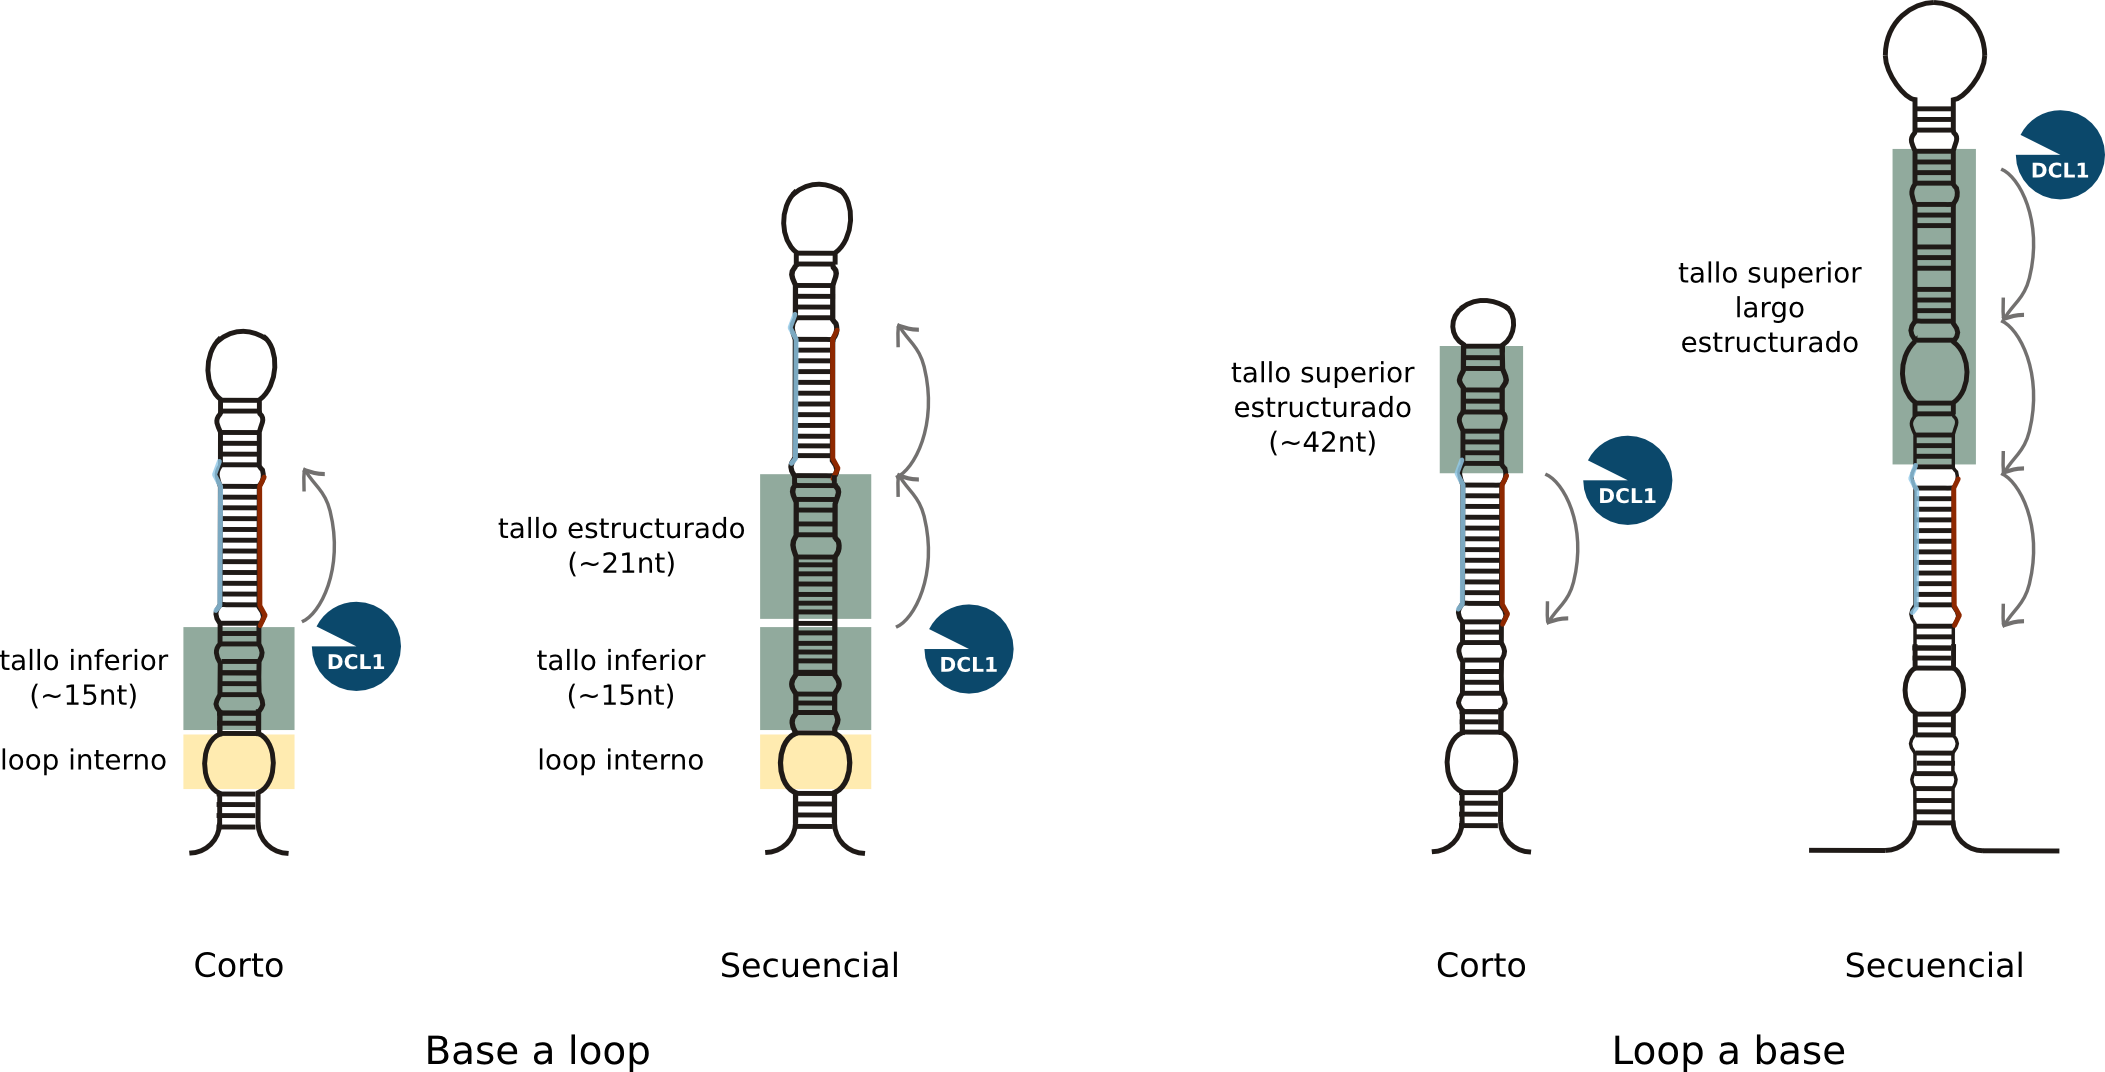
\includegraphics[width=1\textwidth]{mecanismos.png}
    \caption[Mecanismos de procesamiento]{Distintos mecanismos de procesamientos de miARNs en plantas}
    \label{fig:mecanismos}
\end{figure}


%~ ################################################# 
%~ Identificación de intermediarios de procesamiento
%~ en plantas mutantes en proteínas de procesamiento
%~ #################################################

\subsection{Identificación de intermediarios de procesamiento en plantas mutantes en proteínas de procesamiento}

La técnica de SPARE (del inglés Specific Parallel Analisys of 5'RNA Ends) fue desarrollada con el objetivo de caracterizar el procesamiento de los precursores de miARNs de \textit{A. thaliana}.
Para esto se identifican los intermediarios de procesamiento de cada uno de dichos precursores, y uniendo la información brindada por los diferentes fragmentos es posible dilucidar tanto la dirección, como el número de cortes requeridos para la biogénesis de cada miARN (Figura \ref{fig:SPARE_tecnica}).

\begin{figure}[htbp!] 
	\centering    
	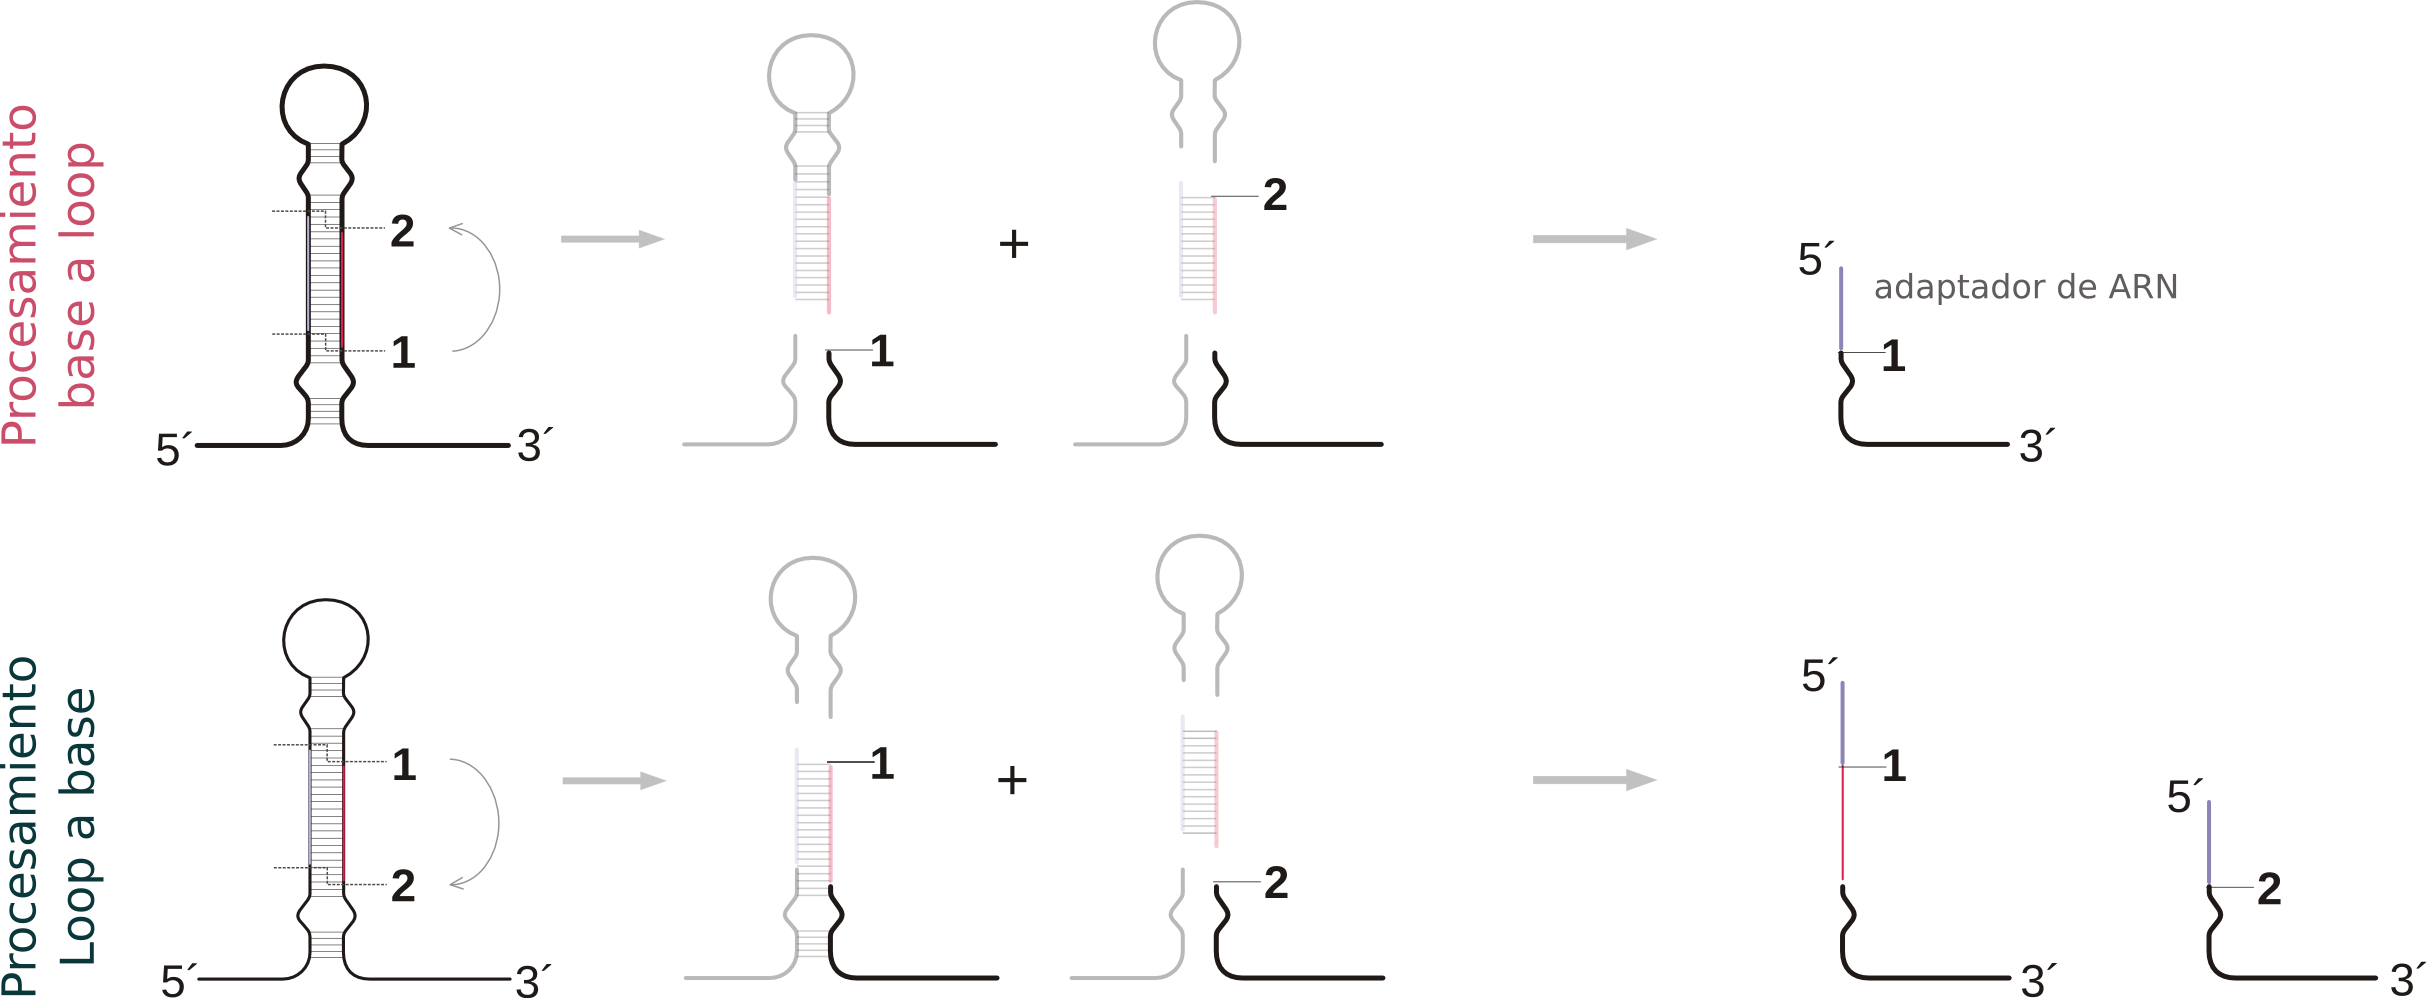
\includegraphics[width=1\textwidth]{SPARE_tecnica.png}
	\caption[Técnica de SPARE]{Técnica de SPARE para diferenciar mecanismos de procesamiento de precursores.
	Detalle donde se muestra a nivel molecular como la técnica permite diferenciar entre dos direcciones de procesamiento opuestas. }
	 \label{fig:SPARE_tecnica}
\end{figure}

Brevemente la técnica consiste en emplear los extremos 5'P dejados por la maquinaria de procesamiento en los precursores luego del clivaje para realizar una ligación ARN-ARN entre los intermediaros de procesamiento y un oligo de ARN de secuencia conocida.
A continuación se emplean oligos específicos para retro-transcribir los intermediaros de cada precursor en particular, con una cola común a todos.
En este punto todos los fragmentos generados durante el procesamiento presentan los mismos extremos: en el 5' la secuencia del oligo de ARN y el en el extremo 3' la secuencia común incorporada durante la retro-transcripción.
Esta información es empleada para diseñar oligos (FW y RV) que se emplean en una reacción de PCR a continuación.
Finalmente los fragmentos son secuenciados. 

En la sección \ref{sec:procesamiento} mostramos los resultados obtenidos de esta técnica para determinar la dirección de procesamiento de los precursores de miARNs en plantas.
Esta nueva secuenciación se realizó debido que anteriormente no se pudieron de determinar la dirección de procesamiento de algunos precursores.
Además, en esta nueva tanda de secuenciación de precursores se intentó identificar intermediarios de procesamiento en plantas mutantes en proteínas de procesamiento.  
Para esta parte del trabajo se hicieron algunas modificiaciones de la técnica.
Se ubicaron los oligos a 100 nt del último corte 3' esperado.
En total se diseñaron 121 oligos para retrotranscribir el conjunto de precursores conservados y jóvenes validados hasta el momento.  
Además, anteriormente el procesamiento de los datos a partir de los datos crudos se hicieron en el mismo laboratorio que se realizaron las secuenciaciones.

\subsubsection{Construcción de bibliotecas multiplex}
El paso final consiste en secuenciar las bibliotecas construidas, sin embargo la secuenciación es costosa haciendo económicamente dificultoso secuenciar varias bibliotecas en paralelo para comparar entre diferentes condiciones (siendo este nuestro objetivo con las plantas mutantes en proteínas de procesamiento).
En los últimos años se han desarrollado métodos que hacen posible secuenciar más de una biblioteca por calle.
Esto consiste en marcar los fragmentos provenientes de cada biblioteca con secuencias especificas (detallado en Materiales y Métodos) y separar informáticamente cada secuencia en la biblioteca de la cual provino a luego de secuenciación.
Técnicamente esto se hace agregando una PCR final donde los índex son incorporados en todas las secuencias de cada biblioteca.

\subsubsection{Diseño experimental}

Con el objetivo de construir bibliotecas de SPARE crecimos plántulas de Arabidopsis thaliana durante 10 días con luz continúa (independizándonos de este modo la variación asociada al ritmo circadiano a la hora de la colecta de muestra).
Se realizó un experimento con plantas mutantes en proteínas de procesamiento.

\textbf{Plantas mutantes en proteínas de procesamiento}

\textit{Hyl1}, \textit{Se} y \textit{Fiery}.
Siendo sus controles plantas silvestres de Arabidopsis ecotipo Col-O.

 
%~ \textbf{Plantas sometidas a diferentes temperaturas}
%~ 
%~ En este caso sólo se utilizaron plantas Col-0 y fiery crecidas en las condiciones descriptas anteriormente y que luego fueron sometidas a un tratamiento de dos horas a tres temperaturas diferentes: 8 \degree C, 22 \degree C y 37 \degree C.
%~ Luego se realizó la colecta de muestra a la temperatura del tratamiento. 

\subsubsection{Herramienta web para el análisis de intermediarios de procesamiento en plantas}

De la técnica de SPARE se obtienen una gran cantidad de datos arrojados por el secuenciador para cada biblioteca secuenciada.
Estos datos se conocen como datos crudos y son fragmentos de secuencia que luego tienen que ser mapeados contra el genoma de datos de interés.
Además, estos datos crudos cuentan con información de las secuencia, lo que permite mediante programas informáticos hacer un control de calidad de la secuencias obtenidas.
En total se obtuvieron cerca de 150 millones de secuencias (Figura \ref{fig:SPARE_estrategia}).

Esos fragmentos son agrupados y mapeados contra las secuencias únicas de los precursores de \textit{A. thaliana}.
Nos quedamos con 7158 secuencias únicas, que luego las filtramos por largo de la secuencia (Figura \ref{fig:SPARE_estrategia}).
Esa información ya procesada es la que utilizamos en la herramienta para analizar y comparar los intermediarios de procesamiento para plantas silvestreste y mutantes de procesamiento.

Para facilitar el análisis de los datos obtenidos por la técnica de SPARE, creamos una herramienta web disponible en la red interna del laboratorio.
La herramienta permite seleccionar un precursor en particular de los $\sim$100 precursores que se detectaron fragmentos por la técnica de SPARE.
Luego se selecciona una o varias mutantes y controles que se quieren analizar.
Además la herramienta permite modificar otros parámetros como la longitud y abundancia de los fragmentos secuenciados a considerar.

\begin{figure}[htbp!] 
	\centering    
	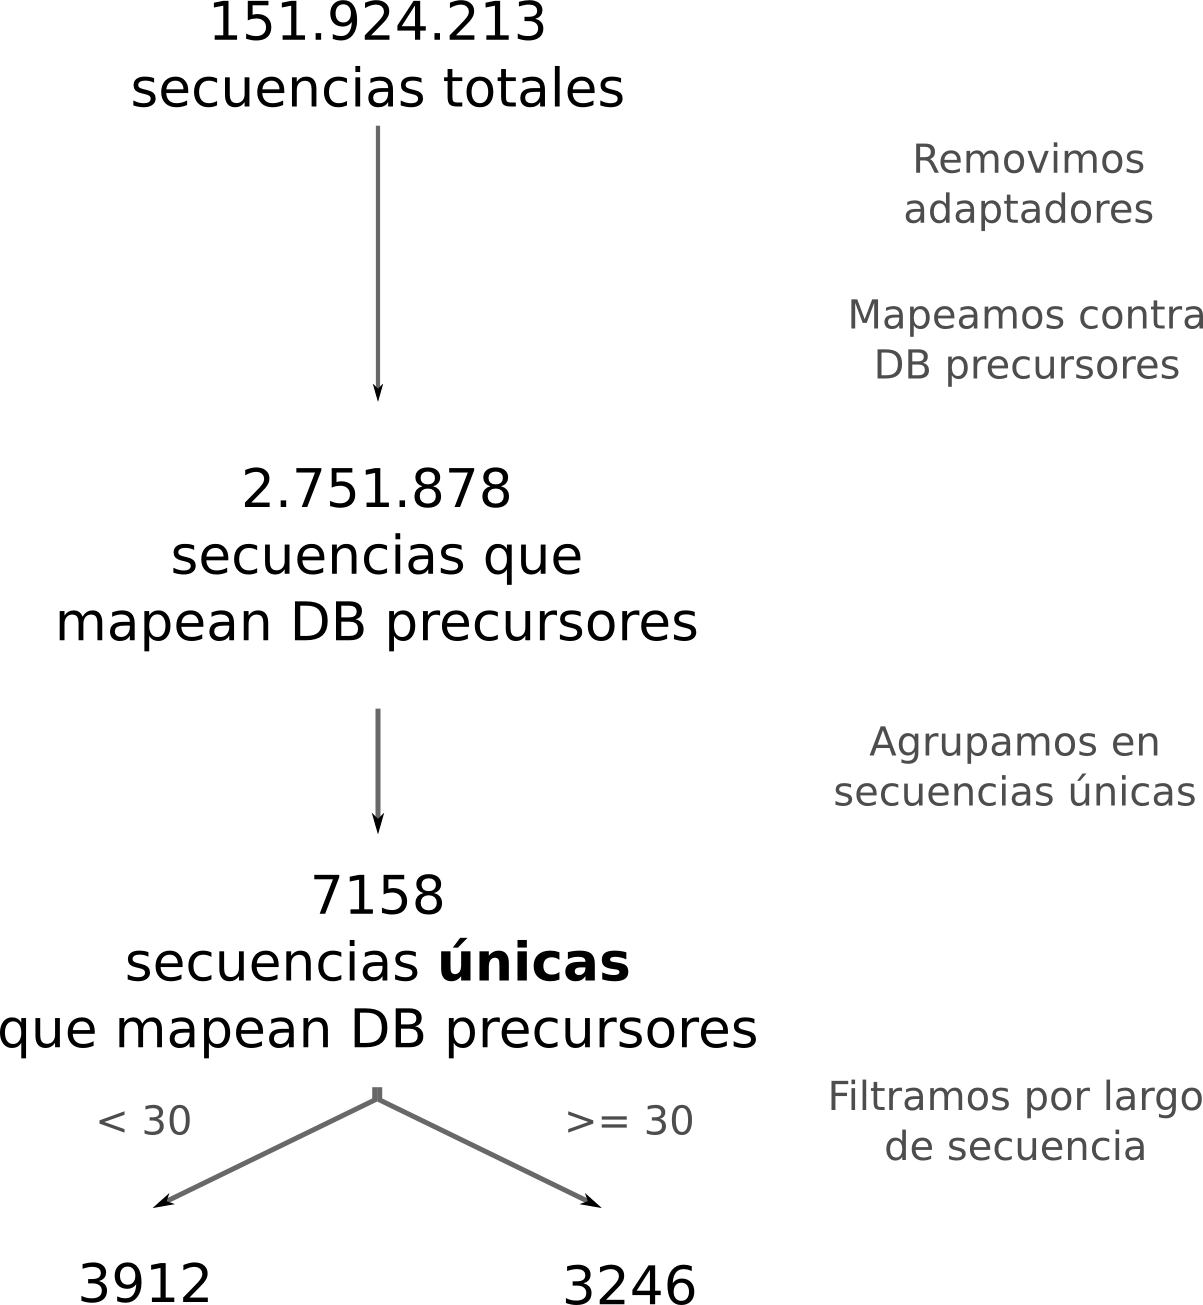
\includegraphics[width=.5\textwidth]{SPARE_estrategia.png}
	\caption[Análisis informático utilizado para procesar los datos de SPARE]{
	Análisis informático utilizado para procesar los datos de SPARE.
	Las secuencias únicas mapeadas contra los precursores son las que se utilizan en la herramienta para analizar los intermediarios de procesamiento.
	}
	 \label{fig:SPARE_estrategia}
\end{figure}

Primero vemos la salida de la herramienta para el precursor del  miR165a, analizando distintas mutantes de procesamiento al mismo tiempo (Figura \ref{fig:miR165a_SPARE}).
La posición final del duplex miARN/miARN* fue considerada como la posición 0, y las posiciones positivas son bases hacia arriba del dúplex mientrás que las posiciones negativas son bases hacia abajo del dúplex.
Los fragmentos se muestran en forma porcentual tomando cada biblioteca de forma independiente y en distintos colores se representan las distintas bibliotecas.
Además se muestra una tabla con los valores absolutos de cada fragmento y con flechas verdes se marcan las posiciones con los fragmentos de mayor abundancia en promedio de todas las bibliotecas (Figura \ref{fig:miR165a_SPARE}).
 
En esta figura se muestra un precursor que es procesado con un mecanismo corto de base a loop, donde según se muestra en la Figura \ref{fig:SPARE_tecnica}, los fragmentos detectados corresponden únicamente al primer corte por DCL1 (Figura \ref{fig:miR165a_SPARE}).
Se pueden observar también cortes en las posiciones $\pm 2$ con respecto a las esperadas por actividad "sloopy" (poco rigurosa) de DCL1 \citep{pmid17989254}.
Además se observan en la posición -5, que aparecen fragmentos en todas las bibliotecas aunque en muy baja abundancia (Figura \ref{fig:miR165a_SPARE}).

Mediante esta herramienta no sólo se puede identificar los precursores procesados de base a loop o de loop a base, sino que también permite identificar a los precursores que denominamos secuenciales, que son los que requieren de más de dos cortes por DCL1 para liberar al miARN maduro.
Por ejemplo, mostramos al precursor del miR169d que es procesado de forma secuencial de base a loop.
En estos precursores, los sitios de cortes delestán localizados 21 nt por debajo del lado proximal del dúplex miARN/miARN* y luego DCL1 sigue cortando para procesar al precursor.
En este caso se detecta un fragmento mayoritario en la posición -21, es decir 21nt por debajo del dúplex miARN/miARN* como era esperado para precursores secuenciales de base a loop \ref{fig:miR169d_SPARE}.

El precursor del miR169d tiene una estructura particular donde presenta un loop ramificado.
Con la herramienta, se puede observar que este precursor particular presenta fragmentos que provienen del corte secuencial de la base al loop que corresponde a la posición -21 en el gráfico.
Pero además, en la mutante de \textit{fiery} se pueden observar fragmentos que corresponden a un corte abortivo por DCL1 a partir del reconocimiento de este loop ramificado \ref{fig:miR169d_SPARE}.
La herramienta permite discriminar este tipo de procesamiento en distintas mutantes de procesamiento. 

\begin{landscape}
    \begin{figure}[htbp!] 
        \centering    
        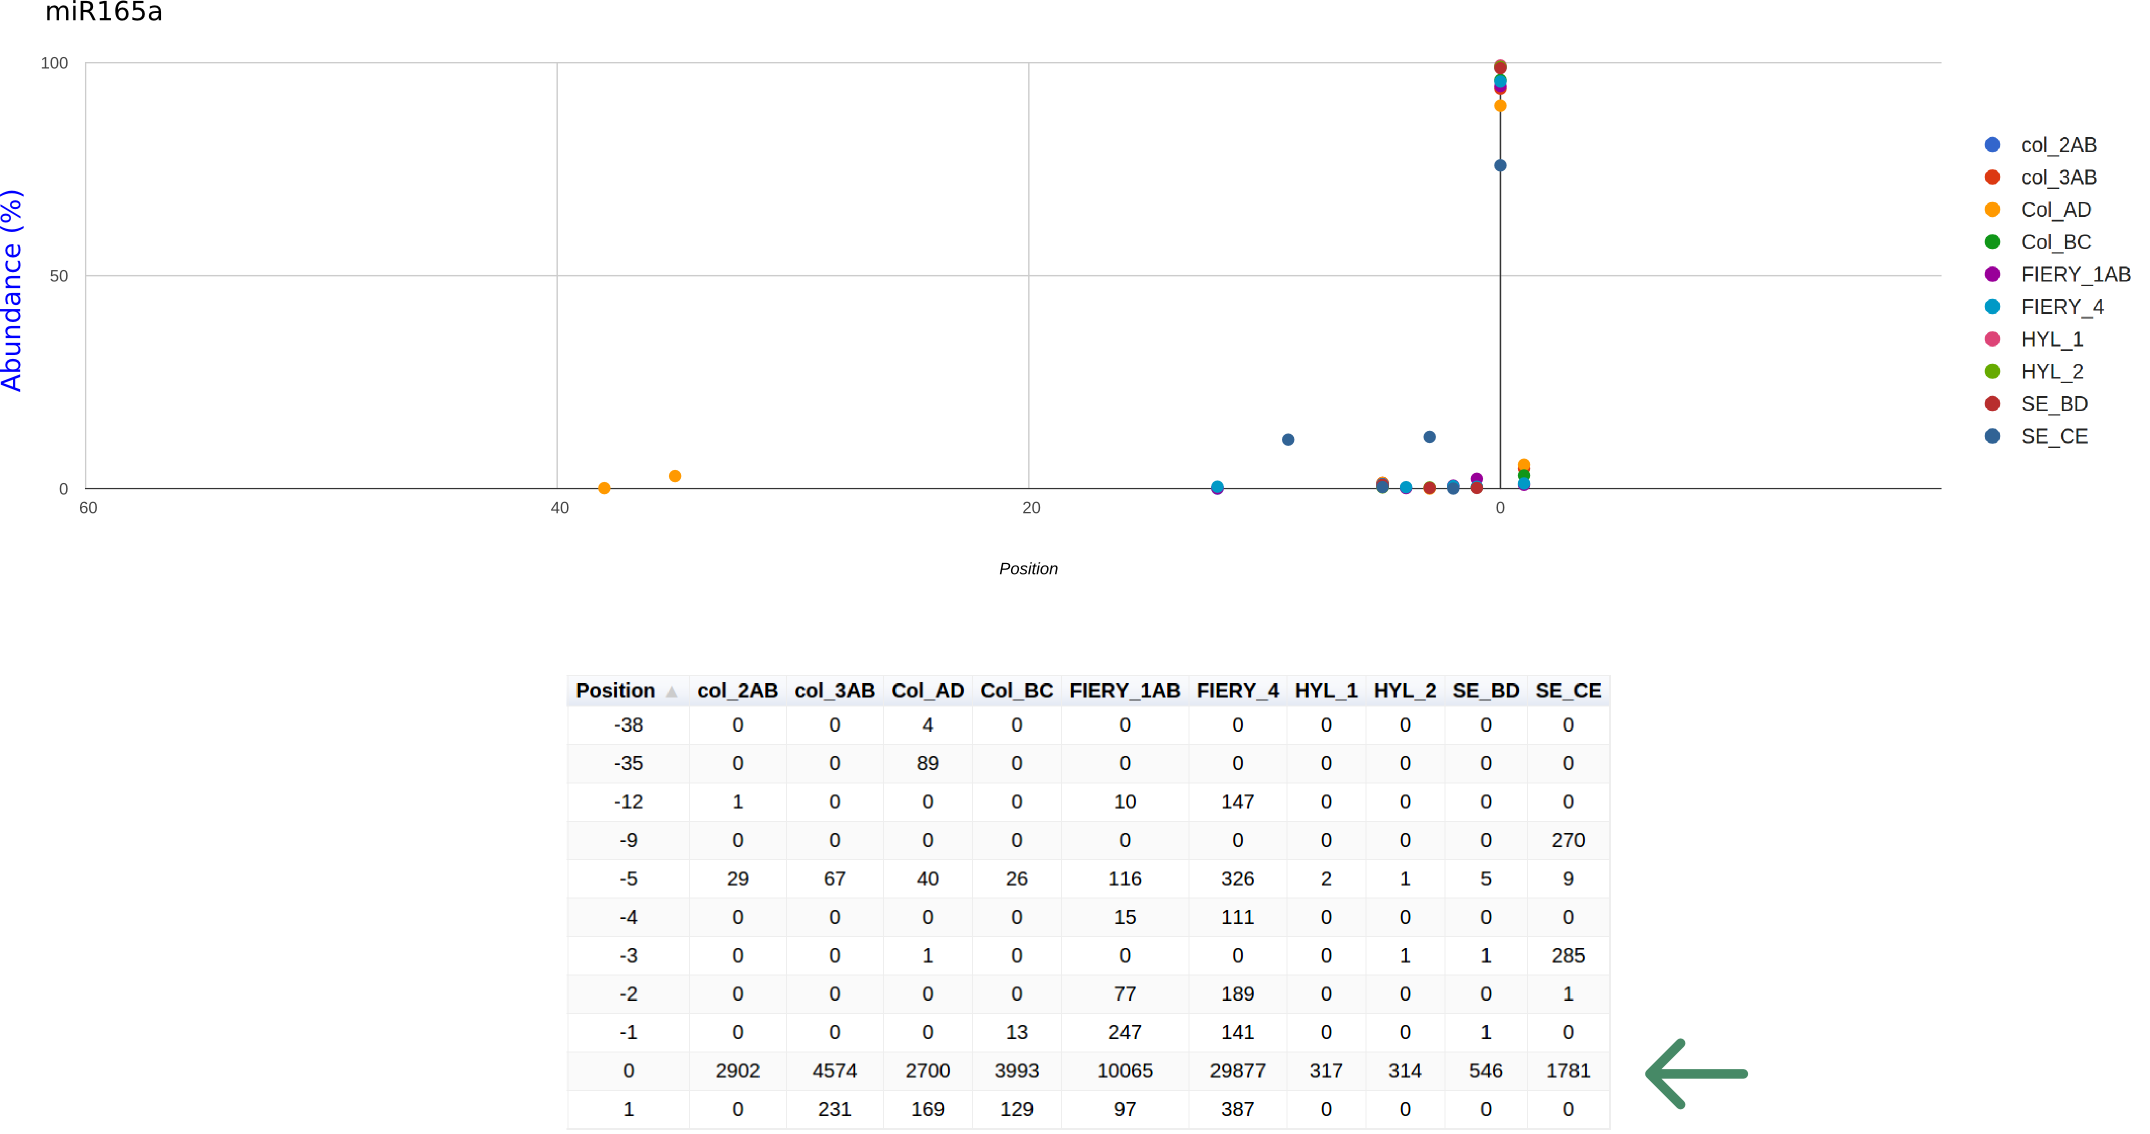
\includegraphics[width=1.4\textwidth]{miR165a_SPARE.png}
        \caption[Captura de pantalla de la herramienta de SPARE para el miR165a]{Captura de pantalla de la herramienta de SPARE para el miR165a.
        Porcentaje de fragmentos del precursor (abundancia relativa de los fragmentos en esa posición dividido la abundancia total de los fragmentos en el precursor).
        La posición final del duplex miARN/miARN* fue considerada como la posición 0.
        La tabla muestra los valores absolutos de cada fragmento.
        Las flechas verdes marcan las posiciones del precursor con los fragmentos de mayor abundancia. 
        }
         \label{fig:miR165a_SPARE}
    \end{figure}
\end{landscape}

\begin{landscape}                                                                      miR169d
\begin{figure}[htbp!] 
        \centering    
        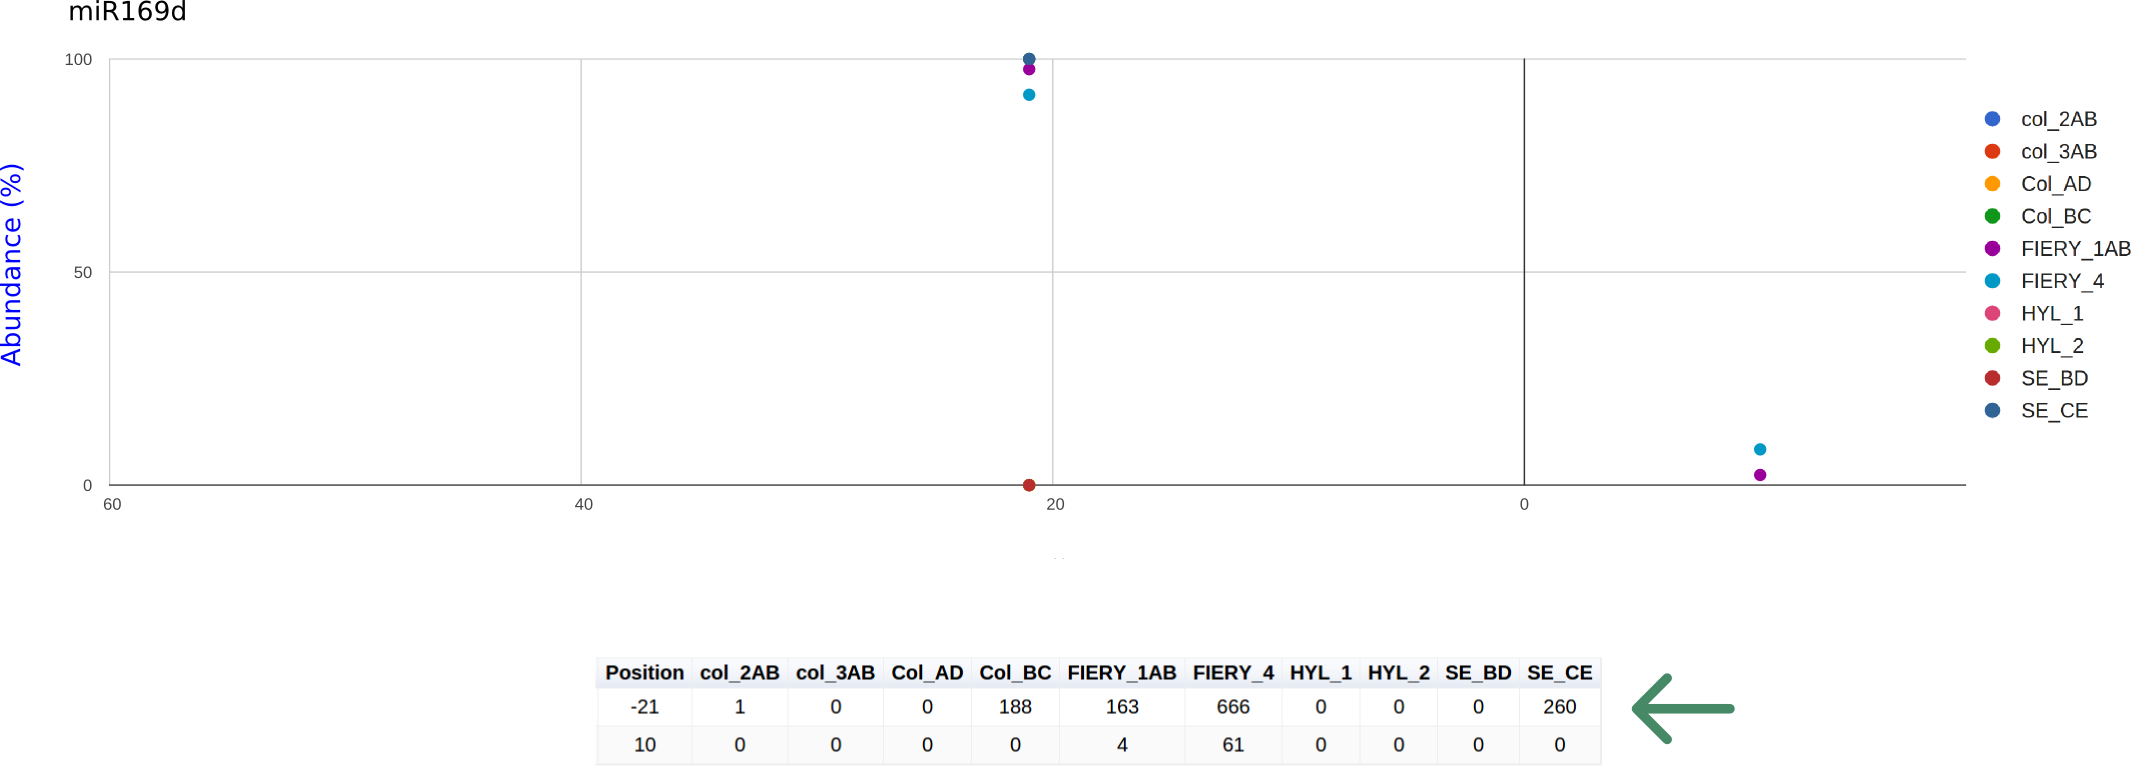
\includegraphics[width=1.4\textwidth]{miR169d_SPARE.png}
        \caption[Captura de pantalla de la herramienta de SPARE para el miR169d]{Capturntalla de la herramienta de SPARE para el miR169d.
        Porcentaje de fragmentos del precursor (abundancia relativa de los fragmentos eosición dividido la abundancia total de los fragmentos en el precursor).
        La posición final del duplex miARN/miARN* fue considerada como la posición 0.
        La tabla muestra los valores absolutos de cada fragmento.
        Las flechas verdes marcan las posiciones del precursor con los fragmentos de mayor abundancia. 
        }
	 \label{fig:miR169d_SPARE}
    \end{figure}
\end{landscape}

Para el caso de los precursores cortos de loop a base, los fragmentos detectados pueden ser más de uno según muestra la técnica de SPARE (Figura \ref{fig:SPARE_tecnica}).
Vemos el precursor del miR156a, donde los cortes más abundantes corresponden a las posiciones 22 y 0 (Figura \ref{fig:miR156a_SPARE}).
Estos fragmentos corresponden a los cortes del precursor por DCL1, donde el primer corte se da en la parte distal del dúplex y el segundo en la parte proximal del mismo.
Además se pueden observar otros fragmentos con abundancias relativas, cercanas a estas posiciones. 
En algunas bibliotecas se puede observar que acumulan más el primer corte (por ejemplo la biblioteca de Col\_AD) y en otras el segundo es el más abundate (biblioteca de Fiery\_1AB) (Figura \ref{fig:SPARE_tecnica}).
Esto podría ser interesante para estudiar en un futuro.
Además se puede observar que en \textit{Hyl} y \textit{Serrate} hay otros fragmentos con abundancia relativa en otras posiciones que las esperadas (posición 3 y posición 14 respectivamente), sugeriendo que tal vez que los cortes podrían estar afectados en estas mutantes de procesamiento (Figura \ref{fig:SPARE_tecnica}).

Por último en el caso del miR159, y al igual que todos los precursores que son procesados secuenciales de loop a base los cuatros fragmentos más abundantes corresponden a los cuatro cortes realizados por DCL1 que son requeridos para procesar este precursor (Figura \ref{fig:miR159b_SPARE}).
El primer corte se da en la posición 71, que de los cuatros cortes es el que tiene fragmentos menos abundantes, y luego DCL1 corta a 21 nucleótidos liberando otros ARN pequeños.
Luego se pueden observar los fragmentos correspondientes al tercer (posición 21) y cuarto corte (posición 0), que son los necesarios para liberar el miARN maduro (Figura \ref{fig:miR159b_SPARE}).
En este caso se pueden ver otros fragmentos que son productos de la degreadación del precursor, aunque nunca son tan abundantes como los fragmentos de los cortes por DCL1.
Por cuestiones de simplicidad, en la tabla solo se muestra los fragmentos con mayor abundancia en promedio de todas las bibliotecas.


\begin{landscape}
    \begin{figure}[htbp!] 
        \centering    
        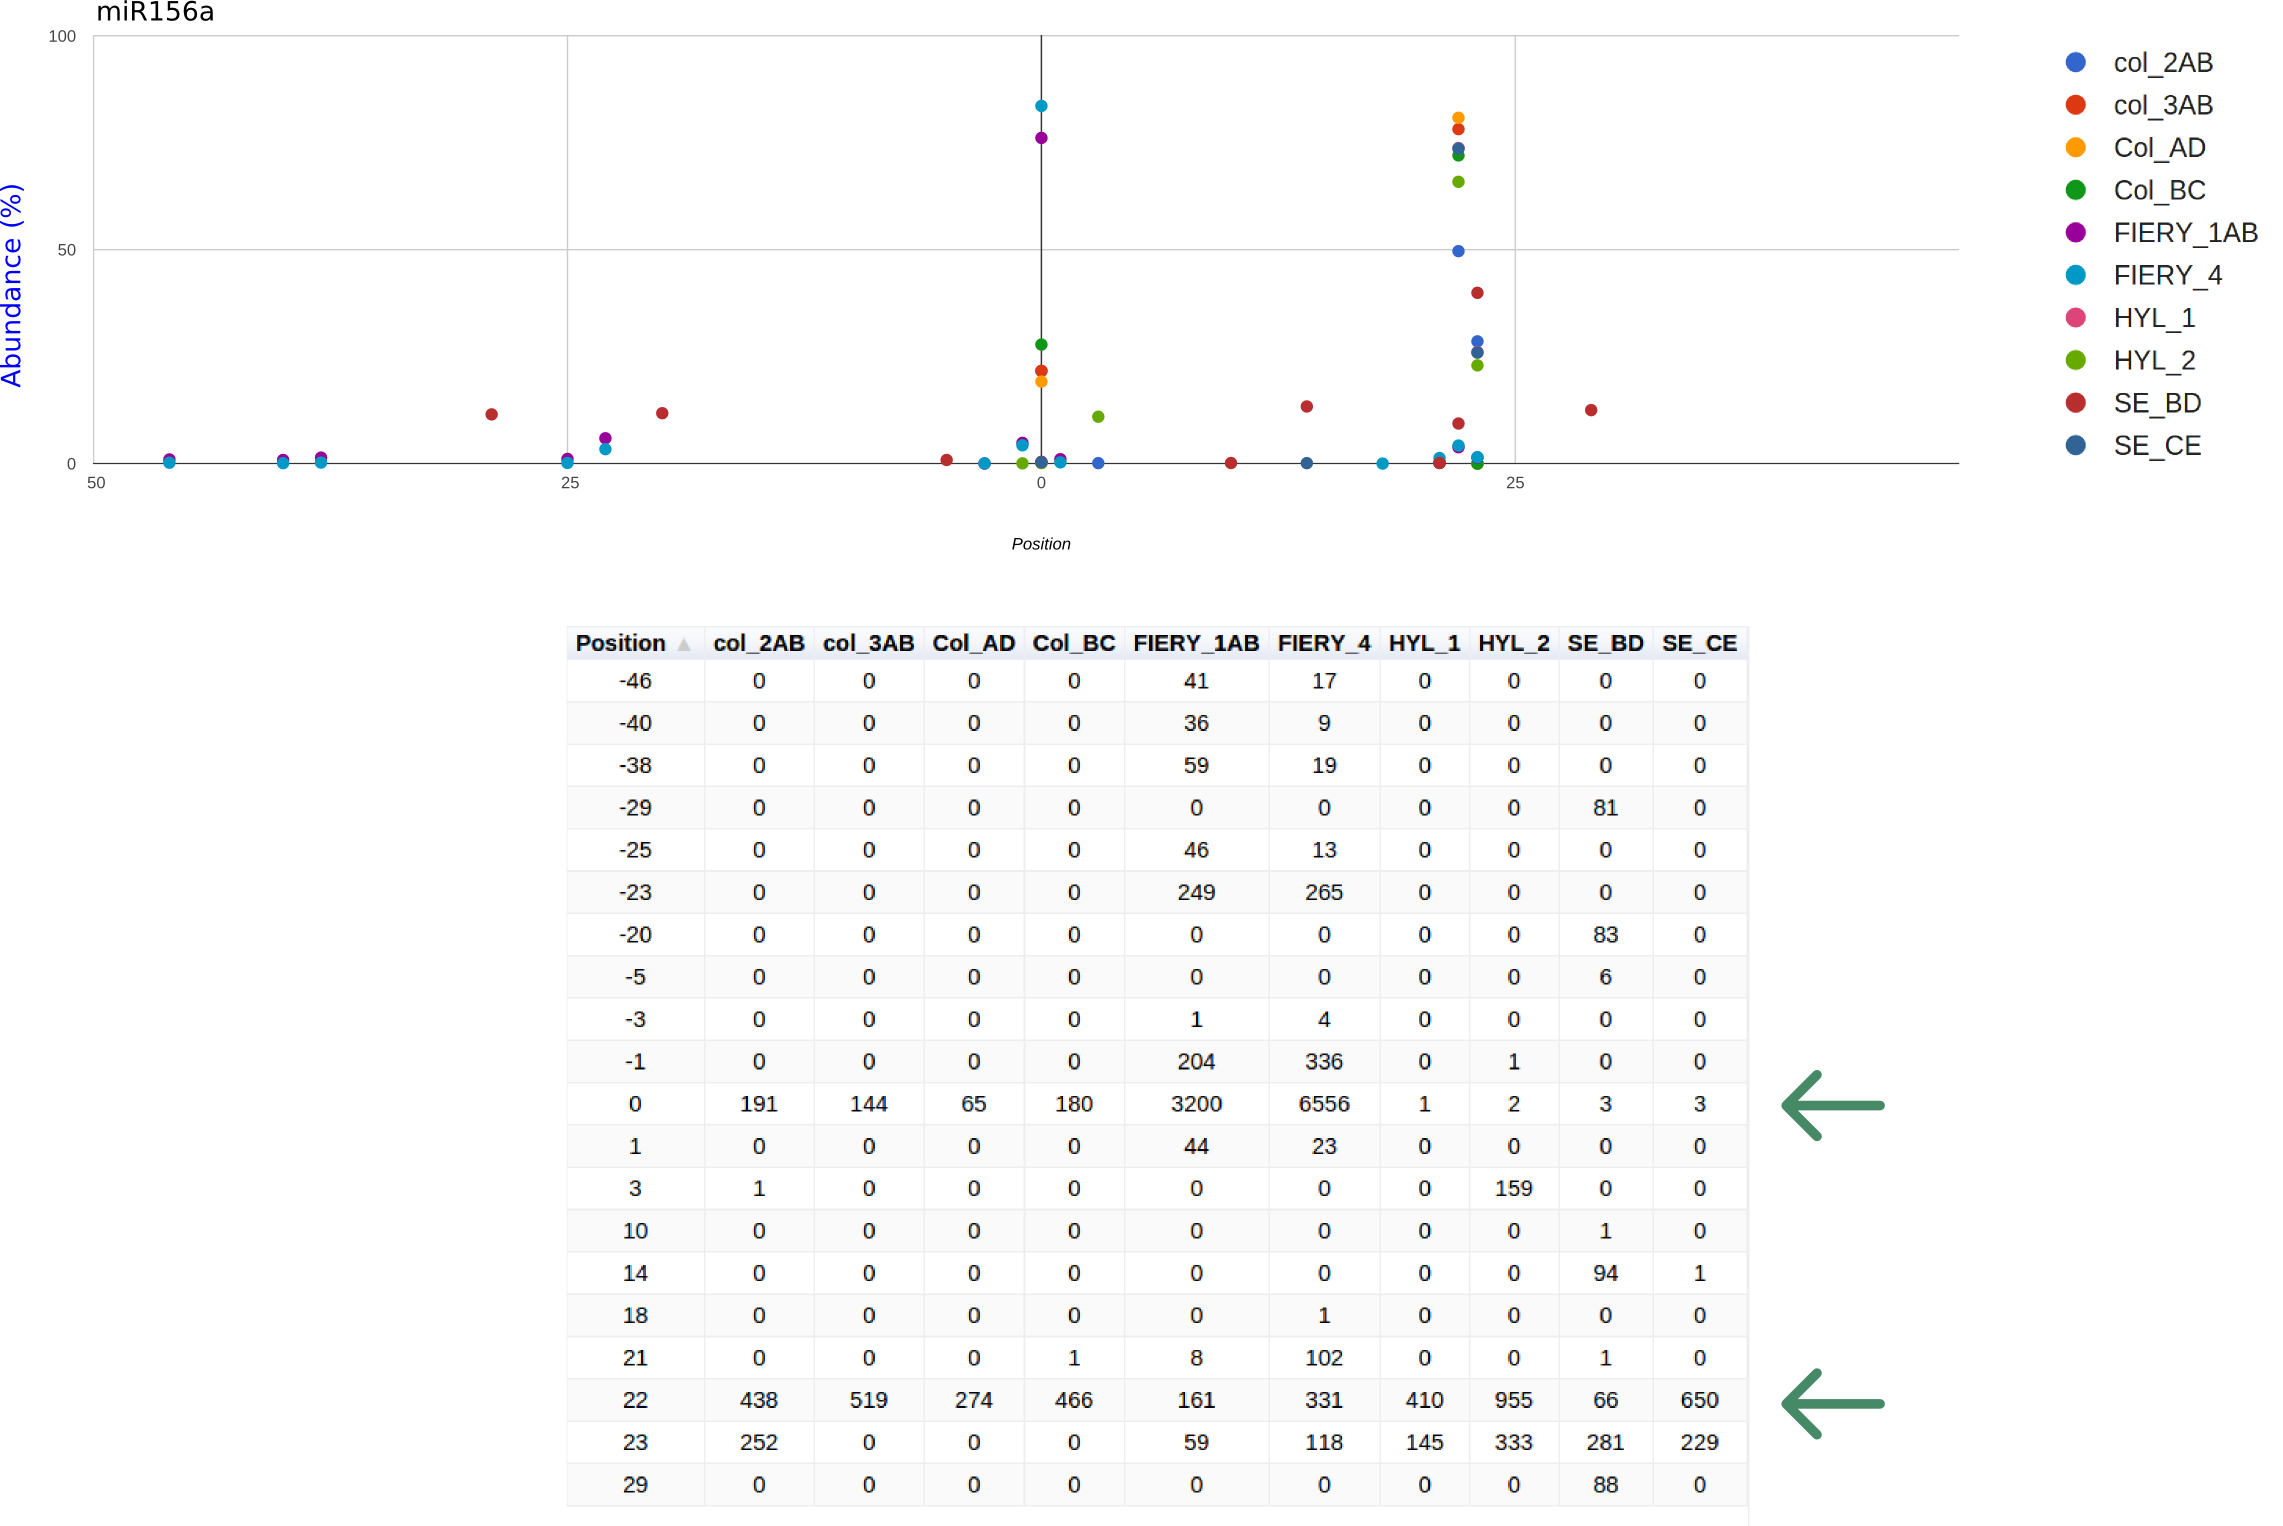
\includegraphics[width=1.4\textwidth]{miR156a_SPARE.png}
        \caption[Captura de pantalla de la herramienta de SPARE para el miR156a]{Captura de pantalla de la herramienta de SPARE para el miR156a.
        Herramienta para analizar los datos de la técnica SPARE.
        Porcentaje de fragmentos del precursor (abundancia relativa de los fragmentos en esa posición dividido la abundancia total de los fragmentos en el precursor).
        La posición final del duplex miARN/miARN* fue considerada como la posición 0.
        La tabla muestra los valores absolutos de cada fragmento.
        Las flechas verdes marcan las posiciones del precursor con los fragmentos de mayor abundancia. 
        }
         \label{fig:miR156a_SPARE}
    \end{figure}
\end{landscape}



\begin{landscape}
    \begin{figure}[htbp!] 
        \centering    
        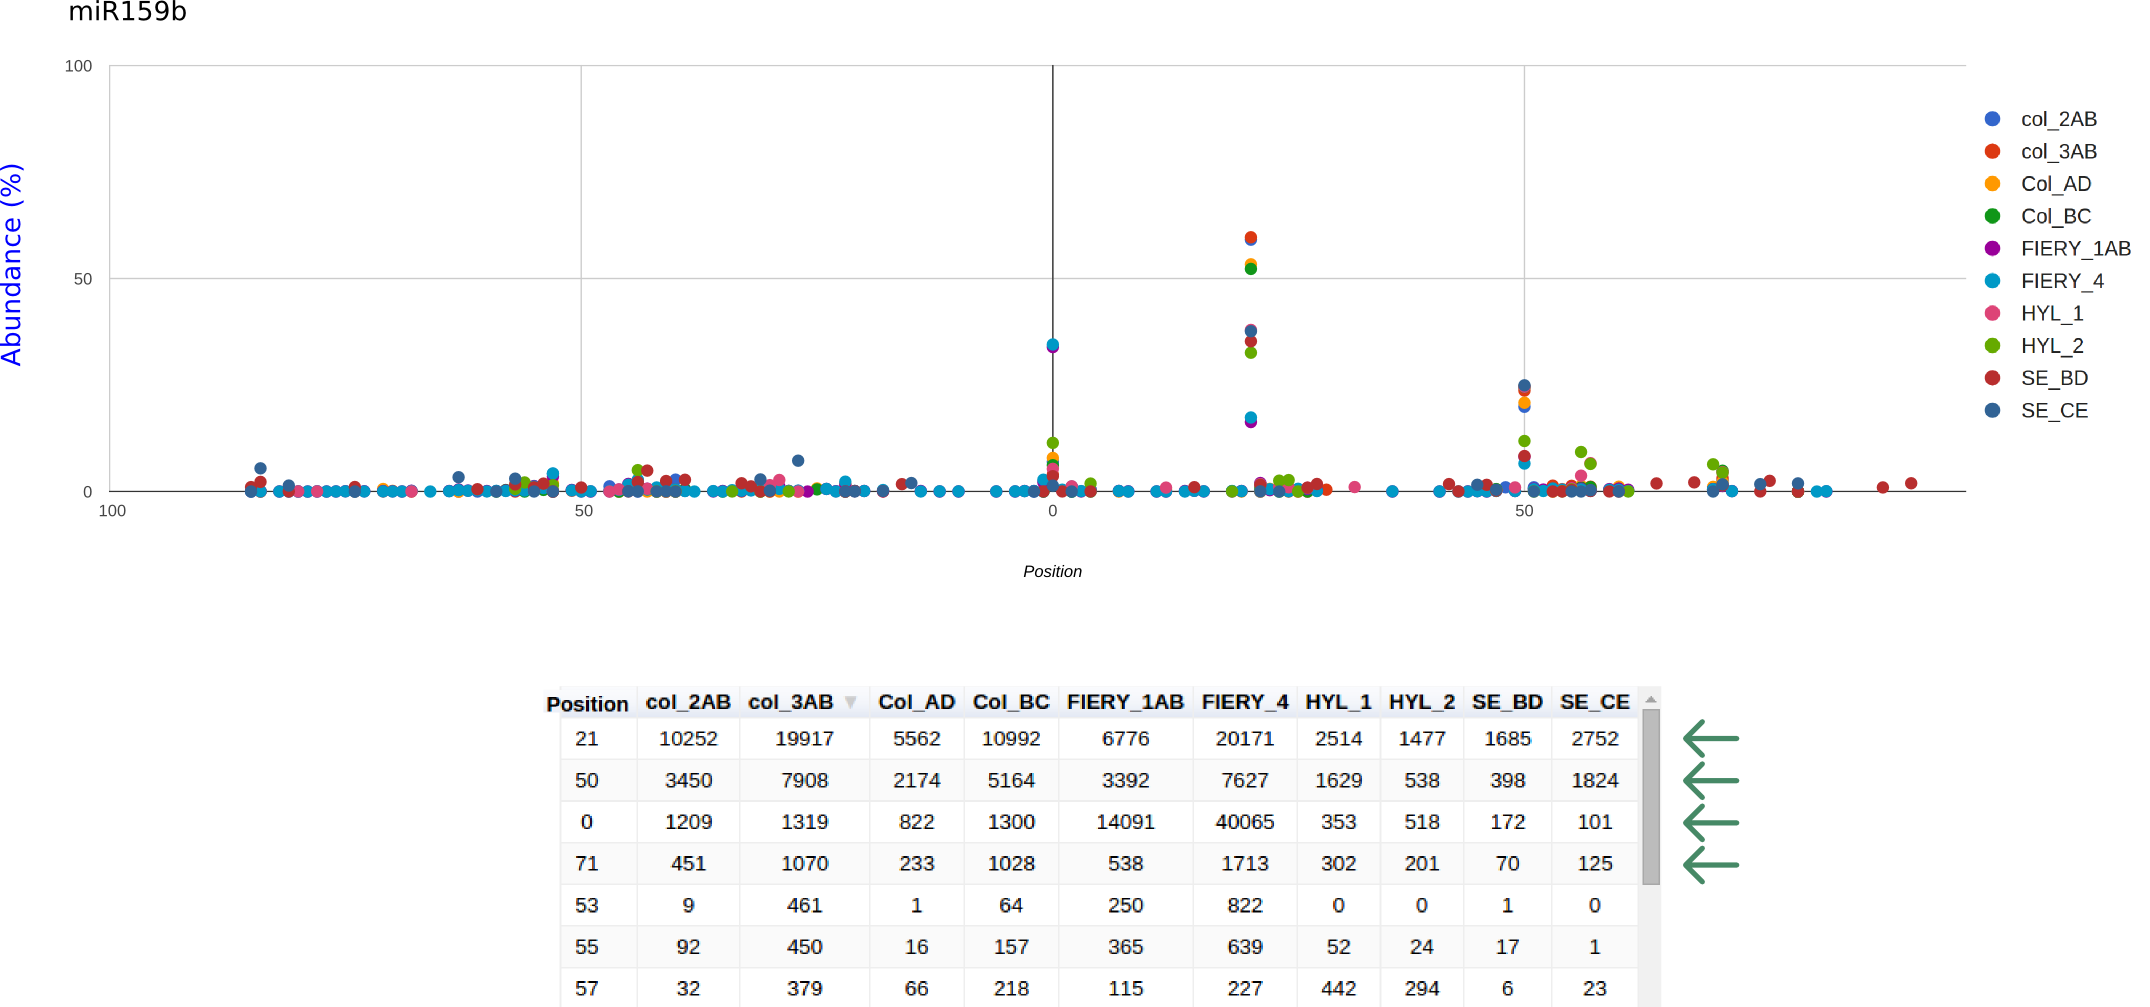
\includegraphics[width=1.4\textwidth]{miR159b_SPARE.png}
		\caption[Captura de pantalla de la herramienta de SPARE para el miR159b]{Captura de pantalla de la herramienta de SPARE para el miR159b.
        Porcentaje de fragmentos del precursor (abundancia relativa de los fragmentos en esa posición dividido la abundancia total de los fragmentos en el precursor).
        La posición final del duplex miARN/miARN* fue considerada como la posición 0.
        La tabla muestra los valores absolutos de cada fragmento.
        Por cuestiones de simplicidad, solo se muestran en la tabla los fragmentos con mayor abundancia en promedio de todas las bibliotecas.
        Las flechas verdes marcan las posiciones del precursor con los fragmentos de mayor abundancia.
        }
		\label{fig:miR159b_SPARE}
    \end{figure}
\end{landscape}






% ********************************** Back Matter *******************************
% Backmatter should be commented out, if you are using appendices after References
%\backmatter

% ********************************** Bibliography ******************************
\begin{spacing}{0.9}

% To use the conventional natbib style referencing
% Bibliography style previews: http://nodonn.tipido.net/bibstyle.php
% Reference styles: http://sites.stat.psu.edu/~surajit/present/bib.htm

\bibliographystyle{apalike}
%\bibliographystyle{plainnat} % use this to have URLs listed in References
\cleardoublepage
\bibliography{References/references} % Path to your References.bib file


% If you would like to use BibLaTeX for your references, pass `custombib' as
% an option in the document class. The location of 'reference.bib' should be
% specified in the preamble.tex file in the custombib section.
% Comment out the lines related to natbib above and uncomment the following line.

%\printbibliography[heading=bibintoc, title={References}]


\end{spacing}

% ********************************** Appendices ********************************

\begin{appendices} % Using appendices environment for more functunality

% ******************************* Thesis Appendix A ****************************
\chapter{Anexo} 

\section*{Predicción de genes regulados por microARNs.}

%~ \subsubsection*{For 64bit OS}
%~ \begin{verbatim}
%~ edit $~/.bashrc file and add following lines
%~ PATH=/usr/local/texlive/2011/bin/x86_64-linux:$PATH;
%~ export PATH 
%~ MANPATH=/usr/local/texlive/2011/texmf/doc/man:$MANPATH;
%~ export MANPATH 
%~ INFOPATH=/usr/local/texlive/2011/texmf/doc/info:$INFOPATH;
%~ export INFOPATH
%~ \end{verbatim}

%~ \lstinputlisting[language=Perl]{scripts/patmatch_2013.pl}


\begin{table}
\small
\centering
\caption{Especies y base de datos utilizadas para la búsquedas de genes blanco de miARNs conservados}
\label{table:NAR_table_S2}
\begin{tabular}{lc}
Specie                         & \multicolumn{1}{c}{Database}         \\
\hline 
Allium\_cepa                   & http://compbio.dfci.harvard.edu/tgi/ \\
Aquilegia                      & http://compbio.dfci.harvard.edu/tgi/ \\
Arabidopsis\_thaliana          & http://arabidopsis.org/              \\
Beta\_vulgaris                 & http://compbio.dfci.harvard.edu/tgi/ \\
Brassica napus                 & http://compbio.dfci.harvard.edu/tgi/ \\
Capsicum\_annuum               & http://compbio.dfci.harvard.edu/tgi/ \\
Citrus\_clementina             & http://compbio.dfci.harvard.edu/tgi/ \\
Citrus\_sinensis               & http://compbio.dfci.harvard.edu/tgi/ \\
Coffea\_canephora              & http://compbio.dfci.harvard.edu/tgi/ \\
Euphorbia\_esula               & http://compbio.dfci.harvard.edu/tgi/ \\
Festuca\_arundinacea           & http://compbio.dfci.harvard.edu/tgi/ \\
Glycine\_max                   & http://compbio.dfci.harvard.edu/tgi/ \\
Gossypium                      & http://compbio.dfci.harvard.edu/tgi/ \\
Gossypium\_raimondii           & http://compbio.dfci.harvard.edu/tgi/ \\
Haseolus\_vulgaris             & http://compbio.dfci.harvard.edu/tgi/ \\
Helianthus\_annuus             & http://compbio.dfci.harvard.edu/tgi/ \\
Hordeum\_vulgare               & http://compbio.dfci.harvard.edu/tgi/ \\
Ipomoea\_nil                   & http://compbio.dfci.harvard.edu/tgi/ \\
Lactuca\_sativa                & http://compbio.dfci.harvard.edu/tgi/ \\
Lactuca\_serriola              & http://compbio.dfci.harvard.edu/tgi/ \\
Lotus\_japonicus               & http://compbio.dfci.harvard.edu/tgi/ \\
Malus\_x\_domestica            & http://compbio.dfci.harvard.edu/tgi/ \\
Medicago\_truncatula           & http://compbio.dfci.harvard.edu/tgi/ \\
Mesembryanthemum\_crystallinum & http://compbio.dfci.harvard.edu/tgi/ \\
Nicotiana\_benthamiana         & http://compbio.dfci.harvard.edu/tgi/ \\
Nicotiana\_tabacum             & http://compbio.dfci.harvard.edu/tgi/ \\
Oryza\_sativa                  & http://www.jcvi.org/                 \\
Panicum\_virgatum              & http://compbio.dfci.harvard.edu/tgi/ \\
Petunia\_hybrida               & http://compbio.dfci.harvard.edu/tgi/ \\
Phaseolus\_coccineus           & http://compbio.dfci.harvard.edu/tgi/ \\
Populus                        & http://compbio.dfci.harvard.edu/tgi/ \\
Prunus\_persica                & http://compbio.dfci.harvard.edu/tgi/ \\
Saccharum\_officinarum         & http://compbio.dfci.harvard.edu/tgi/ \\
Secale\_cereale                & http://compbio.dfci.harvard.edu/tgi/ \\
Solanum\_lycopersicum          & http://compbio.dfci.harvard.edu/tgi/ \\
Solanum\_tuberosum             & http://compbio.dfci.harvard.edu/tgi/ \\
Sorghum\_bicolor               & http://compbio.dfci.harvard.edu/tgi/ \\
Theobroma\_cacao               & http://compbio.dfci.harvard.edu/tgi/ \\
triphysaria                    & http://compbio.dfci.harvard.edu/tgi/ \\
Triphysaria\_versicolor        & http://compbio.dfci.harvard.edu/tgi/ \\
Triticum\_aestivum             & http://compbio.dfci.harvard.edu/tgi/ \\
Vitis\_vinifera                & http://compbio.dfci.harvard.edu/tgi/ \\
Zea\_mays                      & http://compbio.dfci.harvard.edu/tgi/
\end{tabular}
\end{table}


\begin{table}
\tiny
\centering
\caption{My caption}
\label{table:NAR_table_S3}
\begin{tabular}{lll}
microRNA      & Target       & ID        \\
miR156/miR157 & SPL          & At1g27370 \\
miR156/miR157 & SPL          & At1g53160 \\
miR156/miR157 & SPL          & At2g33810 \\
miR156/miR157 & SPL          & At3g15270 \\
miR156/miR157 & SPL          & At5g43270 \\
miR156/miR157 & SPL          & At1g69170 \\
miR156/miR157 & SPL          & At2g42200 \\
miR156/miR157 & SPL          & At3g57920 \\
miR156/miR157 & SPL          & At5g50670 \\
miR159/miR319 & TCP          & At1g30210 \\
miR159/miR319 & TCP          & At1g53230 \\
miR159/miR319 & TCP          & At2g31070 \\
miR159/miR319 & MYB          & At3g11440 \\
miR159/miR319 & TCP          & At3g15030 \\
miR159/miR319 & TCP          & At4g18390 \\
miR159/miR319 & MYB          & At5g06100 \\
miR159/miR319 & MYB          & At2g26950 \\
miR159/miR319 & MYB          & At2g32460 \\
miR159/miR319 & MYB          & At5g55020 \\
miR160        & ARF          & At1g77850 \\
miR160        & ARF          & At2g28350 \\
miR160        & ARF          & At4g30080 \\
miR162        & DCL          & At1g01040 \\
miR164        & NAC          & At1g56010 \\
miR164        & NAC          & At3g15170 \\
miR164        & NAC          & At5g07680 \\
miR164        & NAC          & At5g53950 \\
miR164        & NAC          & At5g61430 \\
miR164        & NAC          & At3g12977 \\
miR164        & NAC          & At5g39610 \\
miR166/miR165 & HD-ZIPIII    & At1g30490 \\
miR166/miR165 & HD-ZIPIII    & At1g52150 \\
miR166/miR165 & HD-ZIPIII    & At2g34710 \\
miR166/miR165 & HD-ZIPIII    & At5g60690 \\
miR166/miR165 & HD-ZIPIII    & At4g32880 \\
miR167        & ARF          & At1g30330 \\
miR167        & ARF          & At5g37020 \\
miR168        & AGO          & At1g48410 \\
miR169        & HAP2         & At1g17590 \\
miR169        & HAP2         & At1g54160 \\
miR169        & HAP2         & At1g72830 \\
miR169        & HAP2         & At3g05690 \\
miR169        & HAP2         & At3g20910 \\
miR169        & HAP2         & At5g06510 \\
miR170/miR171 & SCL          & At2g45160 \\
miR170/miR171 & SCL          & At3g60630 \\
miR170/miR171 & SCL          & At4g00150 \\
miR172        & AP2          & At2g28550 \\
miR172        & AP2          & At4g36920 \\
miR172        & AP2          & At5g60120 \\
miR172        & AP2          & At5g67180 \\
miR172        & AP2          & At2g39250 \\
miR172        & AP2          & At3g54990 \\
miR390/miR391 & TAS3         & At3g17185 \\
miR390/miR391 & TAS3         & At5g49615 \\
miR390/miR391 & TAS3         & At5g57735 \\
miR393        & TIR1/AFB     & At1g12820 \\
miR393        & bHLH         & At3g23690 \\
miR393        & TIR1/AFB     & At3g26810 \\
miR393        & TIR1/AFB     & At3g62980 \\
miR393        & TIR1/AFB     & At4g03190 \\
miR394        & F-Box        & At1g27340 \\
miR395        & APS          & At3g22890 \\
miR395        & AST          & At5g10180 \\
miR395        & APS          & At5g43780 \\
miR395        & APS          & At4g14680 \\
miR396        & GRF          & At2g22840 \\
miR396        & GRF          & At2g36400 \\
miR396        & GRF          & At2g45480 \\
miR396        & GRF          & At4g24150 \\
miR396        & GRF          & At4g37740 \\
miR396        & GRF          & At5g53660 \\
miR396        & GRF          & At3g52910 \\
miR397        & LAC          & At2g29130 \\
miR397        & LAC          & At2g38080 \\
miR397        & LAC          & At5g60020 \\
miR398        & CSD          & At1g08830 \\
miR398        & CSD          & At2g28190 \\
miR398        & CytC oxidase & At3g15640 \\
miR399        & E2-UBC       & At2g33770 \\
miR399        & E2-UBC       & At2g33770 \\
miR408        & LAC          & At2g30210 \\
mir408        & PLC          & At2g02850 \\
miR827        & SPX          & At1g02860
\end{tabular}
\end{table}





\end{appendices}

% *************************************** Index ********************************
\printthesisindex % If index is present

\end{document}
